%% ----------------------------------------------------------------
%% Thesis.tex -- MAIN FILE 
%% ---------------------------------------------------------------- 

% Set up the document
\documentclass[a4paper, 11pt, oneside]{Thesis}  % Use the "Thesis" style, based on the ECS Thesis style by Steve Gunn
\graphicspath{Figures/}  % Location of the graphics files (set up for graphics to be in PDF format)
% Table configuration packages
\usepackage{array,graphicx}
\usepackage{booktabs}
\usepackage{pifont}
\usepackage{libertine}
\usepackage{tabu}
\usepackage{longtable}
\usepackage{xcolor}
\usepackage{tcolorbox}
\usepackage{textcomp}
\usepackage{multicol}
\usepackage{amsmath}
\usepackage{empheq}
\usepackage{pgfplots}
\usepackage[export]{adjustbox}
\makeatother

% Include any extra LaTeX packages required
\usepackage[square, numbers, comma, sort&compress]{natbib}  % Use the "Natbib" style for the references in the Bibliography
\usepackage{verbatim}  % Needed for the "comment" environment to make LaTeX comments
\usepackage{float} % To keep figures in place
\hypersetup{urlcolor=black, colorlinks=false, pdfborder = {0 0 0}}  % Colours hyperlinks in blue
% Define enumerated description lists
\usepackage{enumitem}
\newcounter{descriptcount}
\newcounter{descriptcount2}
\newlist{enumdescript}{description}{2}
\setlist[enumdescript,1]{%
  before={\setcounter{descriptcount}{0}%
          \renewcommand*\thedescriptcount{\arabic{descriptcount}.}}
  ,font=\bfseries\stepcounter{descriptcount}\thedescriptcount~
}
\setlist[enumdescript,2]{%
  before={\setcounter{descriptcount2}{0}%
          \renewcommand*\thedescriptcount{\roman{descriptcount2}.}}
  ,font=\bfseries\stepcounter{descriptcount2}\thedescriptcount~
}
 

 
%% ----------------------------------------------------------------
\begin{document}
\def\Author{Emmanouil Kalyvas}
\def\ThesisTitle{Using blockchain technology for secure, transparent and traceable energy asset exchange}
% For changes in supervisor, degree type, research group, etc. please change the Thesis.cls file
\frontmatter      % Begin the book's numbering; frontpage
%\pagenumbering{arabic}

% Set up the Title Page
\title  {\ThesisTitle}

\authors  {\texorpdfstring
            {\href{mailto:kalyvase@csd.auth.gr}{\Author - Student ID: 93}}
            {\Author}
            }
\addresses  {\groupname\\\deptname\\\progname\univname}  % Do not change this here, instead these must be set in the "Thesis.cls" file, please look through it instead
\date       {Date}
\subject    {}
\keywords   {}

\maketitle

%% ----------------------------------------------------------------

\setstretch{1.3}  % It is better to have smaller font and larger line spacing than the other way round

% Define the page headers using the FancyHdr package and set up for one-sided printing
\fancyhead{}  % Clears all page headers and footers
\rhead{\thepage}  % Sets the right side header to show the page number
\lhead{}  % Clears the left side page header

\pagestyle{fancy}  % Finally, use the "fancy" page style to implement the FancyHdr headers

%% ----------------------------------------------------------------
% Declaration Page required for the Thesis, your institution may give you a different text to place here
\Declaration{

\addtocontents{toc}{\vspace{1em}}  % Add a gap in the Contents, for aesthetics

I, \Author, declare that this thesis titled, '\ThesisTitle' and the work presented in it are my own. I confirm that:

\begin{itemize} 
\item[\tiny{$\blacksquare$}] This work was done wholly or mainly while in candidature for a research degree at this University.
 
\item[\tiny{$\blacksquare$}] Where any part of this thesis has previously been submitted for a degree or any other qualification at this University or any other institution, this has been clearly stated.
 
\item[\tiny{$\blacksquare$}] Where I have consulted the published work of others, this is always clearly attributed.
 
\item[\tiny{$\blacksquare$}] Where I have quoted from the work of others, the source is always given. With the exception of such quotations, this thesis is entirely my own work.
 
\item[\tiny{$\blacksquare$}] I have acknowledged all main sources of help.
 
\item[\tiny{$\blacksquare$}] Where the thesis is based on work done by myself jointly with others, I have made clear exactly what was done by others and what I have contributed myself.
\\
\end{itemize}
 
 
Signed:\\
\rule[1em]{25em}{0.5pt}  % This prints a line for the signature
 
Date:\\
\rule[1em]{25em}{0.5pt}  % This prints a line to write the date
}
\clearpage  % Declaration ended, now start a new page

%% ----------------------------------------------------------------
% The "Funny Quote Page"
\pagestyle{empty}  % No headers or footers for the following pages

\null\vfill
% Now comes the "Funny Quote", written in italics
\textit{One day or day one. You decide.}

\begin{flushright}
Unknown
\end{flushright}

\vfill\vfill\vfill\vfill\vfill\vfill\null
\clearpage  % Funny Quote page ended, start a new page
%% ----------------------------------------------------------------

% The Abstract Page
\addtotoc{Abstract}  % Add the "Abstract" page entry to the Contents
\abstract{
\addtocontents{toc}{\vspace{1em}}  % Add a gap in the Contents, for aesthetics

This thesis introduces a decentralized energy trading model implemented on a private blockchain network. It leverages blockchain technology in order
to decentralize energy transactions and allow a local network to create its own energy market, controlled by the network participants. It gives the freedom
to energy producers and consumers to make their own energy trading deals and define an energy price that is most convenient to both parties without any intermediates.
These goals are achieved using a local Ethereum blockchain network, a decentralized application build on top of it and a web based user interface where users can interact
with the decentralized application and perform energy transactions. The result of this research is a platform called PowerChain, that can be utilized to facilitated local 
energy transactions using blockchain technology. The source code of the platform is open source and can be found in the following GitHub repository:
\begin{center}
  \url{https://github.com/MnAppsNet/PowerChain}
\end{center}
}

\clearpage  % Abstract ended, start a new page
%% ----------------------------------------------------------------

\setstretch{1.3}  % Reset the line-spacing to 1.3 for body text (if it has changed)

% The Acknowledgements page, for thanking everyone
\acknowledgements{
\addtocontents{toc}{\vspace{1em}}  % Add a gap in the Contents, for aesthetics

I would like to express my sincere gratitude to those who have made this thesis possible. First and foremost, my advisors, Prof. Athina Vakali and George Vlahavas, for their invaluable guidance, encouragement, and expertise throughout my research journey. 
Their insightful feedback and unwavering support were instrumental in shaping this project.
My thanks also extend to Aristotle University of Thessaloniki for providing me with the resources and support I needed to conduct my research.
Finally, I would like to express my deepest gratitude to my family. Their love, encouragement, and understanding throughout this journey were more than words can express. 
I am especially grateful to my beloved wife, who is always by my side, supporting me psychologically in every step.
Without the support and guidance of these individuals, this thesis would not have been possible. I am deeply grateful to all of them.

}
\clearpage  % End of the Acknowledgements
%% ----------------------------------------------------------------

\pagestyle{fancy}  %The page style headers have been "empty" all this time, now use the "fancy" headers as defined before to bring them back


%% ----------------------------------------------------------------
\lhead{\emph{Contents}}  % Set the left side page header to "Contents"
\tableofcontents  % Write out the Table of Contents

%% ----------------------------------------------------------------
\lhead{\emph{List of Figures}}  % Set the left side page header to "List if Figures"
\listoffigures  % Write out the List of Figures

%% ----------------------------------------------------------------
\lhead{\emph{List of Tables}}  % Set the left side page header to "List of Tables"
\listoftables  % Write out the List of Tables

%% ----------------------------------------------------------------
\setstretch{1.5}  % Set the line spacing to 1.5, this makes the following tables easier to read
\clearpage  % Start a new page
\lhead{\emph{Abbreviations}}  % Set the left side page header to "Abbreviations"
\listofsymbols{ll}  % Include a list of Abbreviations (a table of two columns)
{
\textbf{Acronym} & \textbf{W}hat (it) \textbf{S}tands \textbf{F}or \\
\textbf{DER}  & Distributed Energy Resource \\
\textbf{PV}   & Photovoltaic \\
\textbf{P2P}  & Peer to Peer \\
\textbf{P2G}  & Peer to Grid \\
\textbf{VPP}  & Virtual power plant \\
\textbf{CDA}  & Continuous Double Auction \\
\textbf{TDDA} & Time Discrete Double Auction \\
\textbf{BMG}  & Brooklyn Microgrid \\
\textbf{BFT}  & Byzantine fault tolerant  \\
\textbf{PBFT} & Practical Byzantine fault tolerant  \\
\textbf{PoW}  & Proof of Work  \\
\textbf{PoS}  & Proof of Stake  \\
\textbf{PoA}  & Proof of Authority  \\
\textbf{DSO}  & Distribute System Operator  \\
\textbf{MCP}  & Market Clearing Price  \\
\textbf{TTP}  & Trusted Third Party  \\
\textbf{UTXO} & Unspent Transaction Output \\
\textbf{EVM}  & Ethereum Virtual Machine \\
\textbf{wh}   & Watt hour \\
\textbf{kWh}  & kiloWatt hour \\

}

\lhead{}
%% ----------------------------------------------------------------
% End of the pre-able, contents and lists of things
% Begin the Dedication page

\setstretch{1.3}  % Return the line spacing back to 1.3

\pagestyle{empty}  % Page style needs to be empty for this page
\dedicatory{Dedicated to my wife who is always by my side...}

\addtocontents{toc}{\vspace{2em}}  % Add a gap in the Contents, for aesthetics


%% ----------------------------------------------------------------
\mainmatter	  % Begin normal, numeric (1,2,3...) page numbering
\pagestyle{fancy}  % Return the page headers back to the "fancy" style

% Include the chapters of the thesis, as separate files
% Just uncomment the lines as you write the chapters

\chapter{Introduction} \label{introduction}
As the consumer level energy generation solutions become cheaper and more available, new opportunities arise in the energy trading sector. Consumers can produce and trade energy on a 
local network and distribution systems operators (DSO) are utilizing distributed energy resources (DERs) such as rooftop solar photovoltaic units (PV) and wind generators to offer affordable and eco-friendly energy 
solutions.
In the past, electricity distribution primarily adhered to a centralized architecture where a central authority oversaw the distribution of energy generated by 
large-scale power plants, predominantly reliant on non-renewable sources like coal and natural gas. Additionally, the large-scale plants producing energy are usually located outside of
cities and far away from consumers. This leads to a big energy waste during the transfer of energy over long distances.
In recent years, ordinary consumers have begun contributing to energy generation through commercially available renewable energy generation units like rooftop solar PV systems. These consumer-producers, also referred 
to as "prosumers" play a crucial role in energy community microgrids. Microgrids are decentralized systems that empower participants to engage in energy trading within local or regional markets. 
They can operate in both grid-connected (meaning they are also connected with the main power grid) or in island-mode (meaning they are completely 
autonomous). An isolated Microgrid has physical connections between the participants that are used to transfer energy and is not connected to the grid. A microgrid connected to the main 
energy grid can also trade energy virtualy with other migrogrids or remote participants and the actual energy exchange happens though the DSO.
To facilitate regional microgrid transactions, the concept of a "virtual power plant" (VPP) has been introduced. VPPs aggregate the capacities of various DERs, integrating diverse energy 
sources to ensure a reliable energy supply. \cite{Pipattanasomporn2013,cali2019towards,BrooklynMicrogrid}\\
Microgrids enable two types of energy distribution models, peer to peer (P2P) and peer to grid (P2G).
In P2P model, energy is getting transacted internally in the participants of the microgrid, in a local market.
In P2G model, energy is getting transacted from/to the microgrid to/from the energy grid based on the grid energy market.
To construct a decentralized P2P and/or P2G energy distribution model, it is necessary to ensure the four below propertied for the metered data:
\begin{itemize}
\item \textbf{Accuracy} of the logged energy assets.
\item \textbf{Traceability} of the energy transactions, to ensure the origin of the generated energy and the correct flow of transactions.
\item \textbf{Privacy} of each network participant. It shouldn't be possible to identify the total energy bill of a participant.
\item \textbf{Security} of the energy transactions and the transactions ledger to prevent cyber attacks. \cite{Vangulick2023}
\end{itemize}
Based on the above requirements, blockchain seems to be a viable option for the implementation of a decentralized energy distribution system.\\
Blockchain is an open-source, distributed ledger that can record transactions securely
between two parties, in a verifiable and permanent way. The first running blockchain was implemented by Satoshi Nakamoto in 2008
and it was meant to be a P2P electronic cash system \cite{Nakamoto}. % Introduction

\chapter{Fundamentals} \label{fandamentals}
In this chapter, we will delve into the foundational aspects of blockchain technology and P2P energy trading.
Initially, we will clarify the concept of a smart contract and explore its life cycle. Following that, we will introduce the most popular consensus mechanisms
and various blockchain platforms, examining their distinctions. Finally, we will outline the P2P energy trading paradigm,
drawing comparisons with traditional energy trading and we will explore different market clearing methods used on energy trading.

\section{Blockchain Technology}
A blockchain is a digital framework that functions as a decentralized, communal database. Within this framework, there exists an ever-expanding record of transactions
organized chronologically. Essentially, this digital structure operates much like a ledger, capable of housing digital transactions, data records, and executable code.
Transactions are grouped into larger units known as "blocks," each bearing a timestamp and cryptographic connections to prior blocks. This creates a linked sequence of records,
establishing the order of events within the blockchain. Beyond defining the data structure itself, the term "blockchain" is also widely used in academic literature to describe digital consensus
systems, algorithms or application domains that are constructed upon these foundational structures.\\
The primary objective of blockchain technologies is to eliminate the necessity for intermediaries and replace them with a distributed network of digital participants who
collaborate to authenticate transactions and preserve the ledger's integrity. In contrast to centralized systems, each member of the blockchain network maintains their own copy
of the ledger or can access it in the public cloud. Consequently, anyone within the network can access the historical record of system transactions and verify their legitimacy,
promoting a high level of transparency. With the removal of central management, the challenge lies in developing an efficient method to consolidate and synchronize multiple ledger
copies. The precise process of validation and ledger consolidation varies among different types of blockchains. However, in principle, network members compare their ledger versions
through a process resembling distributed voting, ultimately reaching a consensus on the valid ledger state. These validation mechanisms are commonly referred to as distributed
consensus algorithms.\\
\begin{figure}[h!]
    \centering
    \includegraphics[scale=0.4]{Figures/centralised_vs_distributed.png}
    \caption{Centralized VS Distributed transaction systems \cite{andoni2019blockchain}}
\end{figure}\\
Blockchain also uses cryptographic techniques like hash functions and public-key cryptography to secure the ledger. Cryptographic hash functions are mathematical algorithms
or one-way processes that take an input and convert it into a specific-length output, such as a 256-bit string referred to as the hash output. Their effectiveness relies on the
extreme difficulty of recreating the original input data from the hash output alone, ensuring collision resistance. Furthermore, blockchain employ public-key cryptography, an
asymmetric cryptographic system where each user possesses two cryptographic keys, comprised of numeric or alphanumeric characters:
\begin{itemize}
    \item A secret private key
    \item And a public key which can be shared with other network users
\end{itemize}
These keys are mathematically interconnected, permitting information encrypted with one key to be decrypted exclusively by its counterpart. This public-private key cryptography
ensures:
\begin{itemize}
    \item Authentication: The network can verify the sender's identity because only the sender's public key can decrypt the initial message, which is encrypted and digitally signed
          using the sender's private key
    \item Verification that a transaction originates from the claimed source. Messages processed with a recipient's public key can only be decrypted by the intended recipient possessing
          the corresponding private key.
    \item And authorization, confirming that actions are executed by users with the appropriate privileges
\end{itemize}
These security measures, along with other standard communication features such as data integrity and confidentiality, are achieved within blockchain systems through peer-to-peer
communication and advanced cryptographic techniques. \cite{andoni2019blockchain}

\subsection{Smart Contracts}
Blockchain can also be paired with smart contracts, realizing fully their potential. Smart contracts are executable programs capable of modifying a ledger automatically when specific
conditions are fulfilled, often related to honoring agreements between parties. These contracts encode legal terms and constraints in a computer-readable language. They are
self-enforcing and tamper-resistant, eliminating the need for intermediaries and reducing transaction-related costs. \cite{andoni2019blockchain} \\
The life cycle of a smart contract, consists of 4 main phases: \cite{ZHENG2020475}
\begin{enumerate}
    \item Creation of smart contract: Multiple parties negotiation on the rights, obligations and prohibitions of their contract. They reach a common agreement and a smart contract is
          build. The smart contract development is done using a smart contract programming language compatible with the blockchain that will be deployed. The smart contract need to be tests
          vigorously as logical code mistakes could result into a breach of the agreement between the parties and assets could be in danger.
    \item Deployment of smart contract: The contract is deployed on a blockchain platform and can't be modified due to the immutability of the blockchain. The contract can be accessed
          by the parties through the blockchain platform. They can initiate the different actions coded by the contract, like for example locking an amount of digital tokens into the contract
          until a condition is met.
    \item Execution of smart contract: The smart contract in effective, the contract conditions are evaluated and the contract statements are executed when the conditions are met.
    \item Completion of smart contract: After the execution of the smart contract new states of all involved parties are updated and stored in the blockchain. At this stage the digital
          assets are moved between the parties based on the initial agreement.
\end{enumerate}
\begin{figure}[h!]
    \centering
    \includegraphics[scale=0.5]{Figures/smart_contract_life_cycle.png}
    \caption{LifeCycle of a smart contract \cite{ZHENG2020475}}
\end{figure}
The main challenge with the creation of a smart contract comes from the fact that blockchains are immutable. As soon as a contract is deployed on the blockchain it can't be modified.
This is a big challenge for smart contract developers as they need to be sure that everything is going to work as expected from the first try.
So it's very important to perform extensive functional tests on the smart contract code before its deployment. \cite{ZHENG2020475}


\subsection{Public and private blockchain networks}
A blockchain network or system can adopt various rules and system architectures based on its intended functionality and specific use cases. Typically, blockchain systems comprise of
network users and validators. User nodes have the capability to initiate or receive transactions and maintain a copy of the ledger. Validators, in addition to read access privileges,
are tasked with approving ledger modifications and achieving consensus across the network concerning the ledger's valid state. Depending on the system's configuration, there may be
partial or universal access rights and validation rights.\\
Public blockchain systems are open to all internet users, while private blockchains restrict access to authorized participants only. Permissionless ledgers are fully decentralized
and resistant to censorship, allowing any network member to participate in transaction validation. Conversely, permissioned ledgers grant write access rights to specific validator
nodes, making the ledger modification process more controlled. In public and permissionless ledgers, users and validators have no prior knowledge of each other, relying on
game-theoretic equilibria and rewards to encourage collaborative and trustworthy ledger management. This incentive structure often involves the expenditure of resources, such as
computational power, electricity, or penalties, to discourage selfish behavior \cite{andoni2019blockchain} Examples of public blockchains with a permissionless ledger are Bitcoin created by Satoshi Nakamoto
\cite{Nakamoto} and Ethereum which was the first public blockchain that made use of smart contracts, proposed by Vitalik Buterin \cite{wood2014ethereum}.\\
Private and permissioned ledgers, on the other hand, operate with known user identities, similar to "know-your-customer" (KYC) practices. Validator nodes are recognized and trusted
to act honestly, eliminating the need for artificial incentives to ensure system operation. Consequently, private and permissioned ledgers can offer increased speed, flexibility
and efficiency, although this comes at the cost of reduced immutability and censorship resistance \cite{andoni2019blockchain}. The most popular permissioned blockchain is Hyperledger fabric proposed by IBM
\cite{androulaki2018hyperledger}.\\
\begin{table}[h!]
    \centering
    \begin{tabular}{l|ll}
        \textbf{Aspect}  & \textbf{Public Blockchain} & \textbf{Private Blockchain}     \\
        \hline
        Access Control   & Open to anyone             & Restricted access               \\[5pt]
        Permission Level & Permissionless             & Permissioned                    \\[5pt]
        Consensus        & Mainly PoW \& PoS          & Various consensus mechanisms    \\[5pt]
        Participants     & Anyone can join            & Approved participants           \\[5pt]
        Privacy          & Anonymous/Pseudonymous     & Known identities (KYC)          \\[5pt]
        Performance      & Slower due to open access  & Faster due to restricted access \\[5pt]
        Scalability      & Limited                    & Potentially better              \\[5pt]
        Example          & Bitcoin, Ethereum          & Hyperledger Fabric              \\[5pt]
    \end{tabular}
    \caption{Public versus private blockchains}
\end{table}

\subsection{Blockchain consensus mechanisms}
In this section, we will present some mechanisms used by blockchain technologies to achieve consensus.
\subsubsection{Proof of Work (PoW)}
The idea behind PoW, as used in Bitcoin, comes from 'Hashcash' which was created to prevent internet resources from being overwhelmed by denial of service attacks.
In PoW, validators or miners compete to add a new block to the existing blockchain by solving a puzzle. They do this by generating a hash that begins
with a certain number of zeros. To achieve this, they add a unique random number (nonce) to the block and calculate the hash of the block's information. This information
includes details like the previous block's hash and a special hash for all the transactions in the block (Merkle tree). Every miner's goal is to produce a hash that's
lower than a specific target value. Since miners can't predict or control the outcome, they have to try different combinations until they succeed. This process requires more
and more computational power as you need more leading zeros. When a miner finally finds the hash that is less than the target, the block is added to the Bitcoin network. Other
nodes check to make sure the transactions are valid and if they are, they accept the newly created block of transactions and the successful miner gets a financial reward.
\cite{andoni2019blockchain}

\subsubsection{Proof of Stake (PoS)}
Proof of Stake, differs from traditional systems by replacing computational work with a random selection method. In PoS, the likelihood of successfully mining a block is
directly linked to the wealth of the validators. The chances of creating a block depend on how much cryptocurrency the nodes have invested in the system, essentially their
coin ownership. This approach potentially allows for faster blockchains with significantly lower electricity consumption and a reduced risk of a 51\% attack.
Unlike other systems, PoS doesn't require the constant creation of new coins to motivate validators. Instead, miners can be rewarded solely with transaction fees, making it
less advantageous to invest heavily in specialized hardware like ASICs.
PoS can also utilize game-theoretical mechanisms to discourage collusion and centralization, often penalizing dishonest or malicious behavior. However, PoS systems face a
primary vulnerability known as the 'nothing at stake' problem. This means that validators can easily vote or claim financial rewards on multiple chains without significant cost.
To address this, various solutions have been proposed, including penalties for validators who create blocks on multiple chains and automatic deductions of owned or deposited
coins. Another approach is to punish validators for creating blocks on the wrong chain, similar in concept to PoW, where validators also incur the cost of electricity.
The latter approach exposes validating nodes to greater risks, but it doesn't require them to be known in advance.
\cite{andoni2019blockchain}

\subsubsection{Practical Byzantine Fault Tolerance (PBFT)}
Byzantine Fault Tolerance (BFT) algorithms find their roots in the study of Byzantine faults, which was initially outlined by Lamport and his colleagues in a significant
computer science paper. To put it simply, this issue revolves around a group of Byzantine generals, or in the context of blockchain, nodes, trying to come to an agreement on
a coordinated course of action. Imagine these generals needing to synchronize their different army units to attack a fortress simultaneously (in the blockchain context, this
means reaching a consensus on whether to validate a block or a set of transactions).
The problem arises because the messages exchanged between these generals must travel through enemy territory, where they could get lost without anyone knowing (think of this
as an unreliable, distributed network). Additionally, some of these generals might be traitors with a vested interest in disrupting the battle plan. They might send false or
distorted messages, or simply not respond to messages at all. The main challenge is to make sure that the loyal generals can agree on the attack plan despite this, and that a
small number of traitors don't lead them to adopt a flawed plan.
In blockchain terms, this means that even if there are a few untrustworthy or potentially malicious nodes, they shouldn't be able to force the validation of a bad block or a
set of transactions.\\
A practical approach for Byzantine Fault Tolerance was introduced by Castro and Liskov \cite{castro1999practical}, for achieving Byzantine Fault Tolerance (BFT) with minimal
computational overhead. Their approach, known as Practical Byzantine Fault Tolerance (PBFT), introduces the concept of primary and secondary replicas. In PBFT, secondary
replicas are responsible for verifying the accuracy and responsiveness of the primary replica and can take over as the new primary if the original primary becomes compromised.\\
PBFT is better suited for use with trusted environment rather than public permissionless ledger. Transactions are signed and verified by known validator nodes and they are
considered valid when a sufficient amount of signatures is reached ans thus also consensus is reached.
\cite{andoni2019blockchain}

\subsubsection{Proof Of Authority (PoA)}
Proof of authority consensus algorithm relays on one or a group of peers to generate new blocks for the network. Network participants holding a special key are responsible to
for generating all network blocks. If the majority of all peer with the special key sign a block, then it's getting accepted into the network. So the network is putting their
trust to a group of authorized peers to generate and validate new blocks. The validators could be elected by a network vote and could be also possible to add new validators with
the same mechanism.
\cite{andoni2019blockchain}

\subsubsection{Comparison of popular consensus mechanisms}

In the table below we compare the different properties of the consensus mechanisms we analyzed in the section above.
Please note that for PoW, 51\% of hash power is regarded as the threshold for one to gain control of the network
but selfish mining strategy in PoW systems could help miners to gain more revenue by only 25\% of the hashing power and thus
the tolerated power of adversary is considered to be 25\%.
\begin{table}[h!]
    \centering
    \begin{tabular}{l|llll}
        \textbf{Aspect}    & PoW            & PoS                & PBFT \& variants   & PoA                \\
        \hline
        Node identity      & Permissionless & Both cases         & Permissioned       & Permissioned       \\
        management         &                &                    &                    &                    \\[5pt]
        \hline
        Energy consumption & High           & Low                & Moderate           & Low                \\[5pt]
        \hline
        Node scalability   & $> 1000$       & $> 1000$           & $< 100$            & $< 100$            \\[5pt]
        \hline
        Transactions per   & 7-30           & 100-200            & up to 110k         & High               \\
        second             &                &                    &                    &                    \\[5pt]
        \hline
        Tolerated power    & $< 25\%$*      & $< 51\%$           & $< 33.3\%$         & $< 51\%$           \\
        of the adversary   & comput. power  & stake              & replicas           & of validators      \\[5pt]
        \hline
        Security           & High           & Depended on        & High within known  & Relied on approved \\
                           &                & participants stake & participants       & authorities        \\[5pt]
        \hline
        Example            & Bitcoin        & Ethereum           & Hyperledger Fabric & VeChain            \\[5pt]
    \end{tabular}\\
    \caption{Comparison of popular consensus algorithms \cite{blockchainTech}}
\end{table}

\pagebreak
\subsection{Blockchain Platforms}
In this section we analyze different available blockchain platforms. Each of the blockchain platforms have different architectures but all of them try to achieve
three main goals:
\begin{itemize}
    \item \textbf{Decentralization}: How censorship resistant is the network, not being able to be controlled or influenced significantly by a small group of network participants.
    \item \textbf{Security}: How secure and robust is the network against attacks from bad actors.
    \item and \textbf{Scalability}: The ability to process transactions, store data and reach consensus as more users are added to the network.
\end{itemize}
It is very difficult to have an architecture that fully achieves these three goals simultaneously. Different approaches improve on two
of the goals in expense of the third. For example, Bitcoin achieves great security and decentralization but it lacks in terms of scalability.

\subsubsection{Bitcoin}
Bitcoin is a public and permissionless blockchain platform that uses the PoW consensus mechanism. Bitcoin protocol makes use of the unspent transaction output (UTXO) model.
In the UTXO model, each transaction has one or more inputs and outputs. The inputs specifies the assets involved in the transaction which must come from a previous transaction output that has not been utilized
in any prior transactions. Meanwhile, the output component is responsible for transferring these assets to a new address. The UTXO model serves a crucial role within the blockchain ecosystem by allowing
network nodes to track the origin of assets involved in any given transaction. This enables them to verify whether the party initiating the transaction possesses the legitimate right to spend those assets.
The movement of assets is recorded in a directed acyclic graph (DAG) between addresses.\\
UTXOs can be owned not only by public keys but also by scripts expressed in simple stack-based programming language. The script requests the data that satisfies the script from a transaction that tries to
spend the UTXO owned by the script. The bitcoin scripting language is not Turing-complete and thus it has limited capabilities not allowing the execution of complex smart-contracts.
\cite{blockchainTech,wang2017novel}
\begin{figure}[h!]
    \centering
    \includegraphics[scale=0.8]{Figures/bitcoin_transactions.png}
    \caption{Bitcoin transactions schematic \cite{Nakamoto}}
\end{figure}\\
Bitcoin network participants can choose to be either clients or miners. Clients are able to send and receive transactions while miners are in charge of creating new blocks through the PoW consensus mechanism.
All network participants keep a copy of the blockchain containing all the recorded transactions and can verify at any time the validity of a transaction.
Transactions are transmitted to the neighboring network peers and are propagated through the network. If the transaction is found to be invalid, it is not broadcasted further to the network and the propagation
stops. Miners store the incoming transaction in a transaction pool if they are valid. A block is constructed out of the transactions in the pool up to the upper block size limit which is about 1 MB. In a UTXO
transactions the input amount can be greater that the output one leaving the rest of the amount as a fee to the miners incentivizing them to prioritize the inclusion of the transaction in the next block.
\cite{blockchainTech,wang2017novel,Nakamoto,UTXOvsACCOUNT}

\subsubsection{Ethereum}
Ethereum is also a public and permissionless platform designed to build and use decentralized applications that run smart contracts. Ethereum smart contracts are written in a fully-fledged Turing-complete programming
language (named Solidity). An Ethereum virtual machine (EVM) is hosted on each network node which is used for the execution of smart contracts. Ethereum was initially relying on the PoW consensus mechanism for the creation of new blocks but it was
later transitioned in PoS.\\
Ethereum uses the account based transaction model where a global ledger is stored and maintained by all network parties based on the PoS consensus. Each block of the blockchain represents a different state of the ledger, this
allows everyone to go through the states of the ledger and validate the origin an legitimacy of a transaction.\\
There are three different account types in Ethereum:
\begin{itemize}
    \item \textbf{Contract Accounts}: A contract account is controlled by code executed by the EVM. They can create transactions with addresses stored in the contract or other contract accounts.
    \item \textbf{Externally Owned Accounts}: These accounts can initiate transactions to transfer Ether to other externally owned accounts, create new contracts or execute functions of existing contract accounts.
    \item \textbf{Miners/Stakers}: They collect unverified transactions, compute a valid state of the ledger, validate transactions, verify signatures and execute code. They collect transactions from the unverified transactions
          pool and compute a new state for the ledger for the next blockchain block choosing transactions based on the fee included in them. They higher the fee the higher the incentive to choose a transaction.
\end{itemize}
When we refer to Ethereum we refer to the open and public Ethereum blockchain network although the Ethereum software is open source and can be also used to create a private blockchain network.
\cite{blockchainTech,ethereum,UTXOvsACCOUNT}

\begin{figure}[h!]
    \centering
    \includegraphics[scale=1.2]{Figures/utxo_vs_account_model.jpg}
    \caption{UTXO VS Account Model \cite{UTXOvsACCOUNT}}
\end{figure}

\subsubsection{Hyperledger}
Hyperledger is an open-source, global ecosystem of enterprise-grade blockchain technologies hosted by The Linux Foundation.
Hyperledger frameworks are designed for permissioned blockchain applications and parties need to be authorized to join the network.
In the hyperledger architecture, the following components are defined:
\begin{itemize}
    \item Consensus Layer: Verify blocks of transactions and agree on the order.
    \item Smart Contract Layer: Processes transactions
    \item Communication Layer: Handles the P2P transport
    \item Data Store Abstraction: Handles different data-stores
    \item Crypto Abstraction: Handles cryptographic algorithms
    \item Identity Service: Registers and authenticates identities of the network
    \item Policy Service: Responsible for policy management
    \item APIs for interaction with other applications
    \item Inter-Operation service: Handles the inter-operation with other blockchain networks
\end{itemize}
Different Hyperledger frameworks have been constructed based on the Hyperledger architecture.
One of the most popular Hyperledger platforms is Hyperledger Fabric.\\
Fabric functions as a distributed operating system designed for permissioned blockchains, running distributed applications that are
coded in widely used programming languages like Go, Java, and Node.js. It maintains a secure record of
its execution history using an immutable replicated ledger data structure, all while lacking any
integrated cryptocurrency. In Fabric, smart contracts are called as Chaincodes and reading or writing the ledger is an operation referred to as a "proposal".
Distributed application within Fabric consists of chaincodes.
A chaincode contains the program code responsible for implementing the application's logic and operates during the execution phase.
Chaincode represents the central element of a distributed application in Fabric and may be authored by a developer whose trustworthiness
is not guaranteed. There are specific chaincodes designed for managing the blockchain system and overseeing
parameters, collectively referred to as system chaincodes.
Fabric nodes can have one of the three roles below:
\begin{itemize}
    \item Client: Submit transaction proposals for execution.
    \item Peers : Execute transaction proposals and validate transactions. All peers has a copy of the blockchain ledger.
          Not all peers can execute all transaction proposals, only endorsing peers can. Execution of a chaincode depends on it's endorsement policy,
          which defines what peers and how many of them can validate it.
    \item  Ordering Service Nodes (OSN): The ordering service receives transactions from all channels in the network, orders them chronologically
          on a per-channel basis, and packages them into blocks. The blocks will be delivered to peers on the channel for final
          validation and commitment. This design choice renders consensus in Fabric as modular as possible and simplifies the replacement
          of ordering service nodes.
\end{itemize}
In a private Fabric network, participants usually reach consensus through the PBFT mechanism.
\cite{blockchainTech,hyperledger}

\pagebreak
\subsubsection{Comparison between blockchain platforms}
In this section we collected all the main differences between the three popular blockchain platforms analyzed above.
In the following table the main characteristics of a blockchain platform are presented along with how each characteristic compares
between the three popular platforms.
\begin{table}[h!]
    \centering
    \begin{tabular}[rounded-corners]{l|lll}
        \textbf{Aspect}         & \textbf{Bitcoin}     & \textbf{Ethereum}          & \textbf{Hyperledger Fabric} \\
        \hline
        Purpose                 & Digital Currency     & Decentralized Apps         & Enterprise blockchain       \\[5pt]
        Target Audience         & Individuals          & Developers, Individuals    & Enterprises, consortiums    \\[5pt]
        Permission Restrictions & Permissionless       & Permissionless             & Permissioned                \\[5pt]
        Access to data          & Public               & Public \& Private          & Private                     \\[5pt]
        Consensus               & PoW                  & PoS                        & PBFT                        \\[5pt]
        Transaction Speed       & Slow (~7/sec)        & Faster (~15-30/sec)        & Moderate speed              \\[5pt]
        Native Currency         & Bitcoin              & Ether                      & None                        \\[5pt]
        Scripting               & Not Turing-Complete, & Turing-Complete,           & Turing-Complete,            \\
                                & Limited Stack-based  & High-Level language        & High-Level languages        \\
                                & scripting            & Solidity                   & Go, NodeJS, Java            \\[5pt]
    \end{tabular}
    \caption{Comparison of popular blockchain platforms}
\end{table}

\subsection{Trusted Authorities}
Blockchain strives for a trustless and decentralized system but there are some aspects that still require some kind of a trusted authority to operate. Such 
example is the bridging of off-chain and on-chain data. A blockchain network has only access to what already exists in the blockchain and is completely isolated. 
In order to bridge off-chain data into the blockchain network, some kind of a trusted authority in needed. Such trusted authorities are also called oracles. Their 
responsibility is to retrieve, verify and feed off-chain data into the blockchain network which can then be used by decentralized applications. Another example of trusted
authority in the blockchain network, is a group responsible of bridging off-chain assets into the blockchain network in the form of a token. Such assets could for example
be a real world currency. The simplest way to achieve this is to store and lock the real world currency (effectively, moving it out of circulation) and minting the relevant amount
of a corresponding token into the blockchain network. With the opposite procedure they can then lock the corresponding blockchain network token and unlock the real world asset.
In general a trusted authority is a middle man that bridges real world data or assets into the blockchain network. The role of a trusted authority can sometimes be replaced by 
algorithms but with a cost on complexity and possibly security of the solution. \cite{oracles}\cite{stablecoins}

\section{P2P Energy Trading}
Energy generation by prosumers can be unpredictable due to different variables which makes it difficult to predict.
Such variables could be the amount of sun for PV units or the wind speed for wind turbines.
In case of energy surplus, a prosumers has three possible options:
\begin{itemize}
    \item To store the energy in batteries considering there is capacity left
    \item Export the excess energy to the electricity grid in market prices
    \item Or sell it to another energy consumer
\end{itemize}
I case of the P2P energy trading model, consumers and prosumers are buying and selling energy directly among them,
on a local energy market, formed by the ask and offered energy prices. In such a local energy trading
market, the network participants first share their generated energy locally and then
trade with the retailers. The local market prices are typically set between the export energy price,
which is the prices the prosumers are selling to the retailers and the retail price, which is the price to buy energy from
retailers. In this way, both prosumers and consumers are benefiting as the former sell energy in a better price while the
latter buy cheaper energy. \cite{Soto2021}

\begin{figure}[h!]
    \centering
    \includegraphics[scale=0.4]{Figures/P2P_Energy_Trading_Model.png}
    \caption{P2P energy trading model \cite{Soto2021}}
\end{figure}

\subsection{Conventional versus P2P energy trade}
In this section, we will discuss what are the benefits of P2P energy trade, what its limitations
and how it compares against the conventional energy trading model. Conventional energy trading is usually one-way,
energy is transmitted from large-scale generators to consumers while cash flow is the other way around, from consumers to
energy providers. The market price can not be influenced directly from the consumers and it is set by energy providers based on market
conditions. In contrast, P2P energy trade is a multi-directional procedures where both the energy and cash, flow between prosumers
and prosumers. The energy price is set by the microgrid based on the participants' bids.
P2P energy trading will also have some impact on the community. It creates new job opportunities for the maintenance and operation
of the P2P systems, it increases social trust as the community works together for their energy needs and generally it creates a great
attachment to the community as the participants have a direct connection with each other. \cite{Soto2021}
\begin{table}[h!]
    \begin{tabular}[rounded-corners]{l|ll}
        \textbf{Aspect} & \textbf{P2P Energy Trade}             & \textbf{Conventional Energy Trade}  \\
        \hline
        Transparency    & High transparency in pricing,         & Less transparent, prices may be     \\
                        & sources and transactions              & influenced by not easily traceable  \\
                        &                                       & sources                             \\[5pt]
        Innovation and  & Relies on blockchain, smart contracts & More traditional infrastructure,    \\
        Technology      & and IoT devices for trading           & slower to adapt new technologies    \\ [5pt]
        Environmental   & Emphasizes renewable energy           & May or may not prioritize           \\
        Impact          & usage, sustainability and             & renewable energy sources            \\
                        & local energy production               & and sustainability                  \\[5pt]
        Regulatory      & Can face hurdles dut to evolving      & Complience with energy policies     \\
        Challenges      & energy market regulations             & and regulations is more established \\[5pt]
        Scalability and & Can be more scalable, efficient and   & May face challenges in adapting to  \\
        Efficiency      & adaptable to localized energy needs   & rapid changes or catering to        \\
                        &                                       & localized demands                   \\[5pt]
    \end{tabular}
    \caption{P2P versus Traditional energy trading}
\end{table}

\subsection{Microgrid Markets}
Apart from the physical connections of a microgrid, there is also a market layer where all the participants' transactions happen.
A microgrid market is usually classified by three main processes :
\begin{itemize}
    \item Identity verification: Verifies the identity of the participant and confirms that he/she can participate in the microgrid market.
    \item Market opening: At market opening, sellers and buyers can submit their bids and the market automatically completes the transactions
          and does the price matching based on the trading rules.
    \item Market closing: The market closes and the participants can't submit any bids until it opens again \cite{wang2017novel}
\end{itemize}

In the following subsections, different market clearing methods will be presented.

\subsubsection{Continuous Double Auction (CDA)}
Most P2P trading platforms are making use of the continuous double auction design for their market layer.
In a CDA market, buyers and sellers can submit their bids at any time of the trading period and
market clears continuously. Buyers' bids are ordered in a descending order, from highest to lowest,
while sellers' bids from lowest to highest. Then a "price first and time first" principle is applied
and the orders are cleared based on the given bids. A CDA market order book example can be seen on the table below. \cite{wang2017novel,DeTrade}

\begin{table}[h!]
    \begin{minipage}[c]{\textwidth}
        \centering
        \begin{tabular}{|c|c|c|c|c|c|}
            \hline
            \multicolumn{6}{|c|}{\textbf{Order Book Before Clearing}}                                                                                               \\
            \hline
            \multicolumn{3}{|c|}{\textbf{Buy Orders}} & \multicolumn{3}{|c|}{\textbf{Sell Orders}}                                                                  \\
            \hline
            Buyer                                     & Requested Price                            & Provided energy & Seller & Requested Price  & Requested energy \\
                                                      & units per energy                           & energy units    &        & units per energy & units            \\
                                                      & unit                                       &                 &        & unit             &                  \\
            \hline
            B1                                        & 10,5                                       & 5               & S1     & 10,2             & 3                \\
            B2                                        & 10,0                                       & 3               & S2     & 10,5             & 1                \\
            B3                                        & 9,9                                        & 4               & S3     & 10,8             & 4                \\
            B4                                        & 9,8                                        & 5               & S4     & 11,1             & 3                \\
            \hline
        \end{tabular}
    \end{minipage}\\
    \begin{minipage}[c]{\textwidth}
        \centering
        \begin{tabular}{|c|c|c|c|c|c|}
            \hline
            \multicolumn{6}{|c|}{\textbf{Order Book After Clearing}}                                                                                                \\
            \hline
            \multicolumn{3}{|c|}{\textbf{Buy Orders}} & \multicolumn{3}{|c|}{\textbf{Sell Orders}}                                                                  \\
            \hline
            Buyer                                     & Requested Price                            & Provided energy & Seller & Requested Price  & Requested energy \\
                                                      & units per energy                           & energy units    &        & units per energy & units            \\
                                                      & unit                                       &                 &        & unit             &                  \\
            \hline
            B1                                        & 10,5                                       & 1               & S3     & 10,8             & 3                \\
            B2                                        & 10,0                                       & 3               & S4     & 11,1             & 1                \\
            B3                                        & 9,9                                        & 4               &        &                  &                  \\
            B4                                        & 9,8                                        & 5               &        &                  &                  \\
            \hline
        \end{tabular}
    \end{minipage}
    \caption{Order book in CDA market, before and after clearing}
\end{table}

The higher bid of a buyer is called the outstanding bid while the higher bid of a seller is called outstanding ask. When the outstanding bid is less or equal to the outstanding
ask, a transaction is happening with the transaction price being equal to the average of the two prices. This process continues until there the outstanding bid is more than the
outstanding ask. This process is called one round of transactions and at least one transaction occurs during that process. In the above table we can see that one round of transactions
is performed which includes two transactions, the one between B1 and S1 for 3 energy units and the one from B1 to S2 for 1 energy unit. \cite{wang2017novel}

\subsubsection{Time Descrete Double Auction (TDDA)}

In a TDDA market, transaction happens at discrete time intervals rather than continuously. Specific time intervals are specified when the participants can make their buying or selling
bids. At the end of this time interval, the system matches buy and sell order based on the outstanding bids and the outstanding asks, like the CDA market. TTDA is more or less and
extension of CDA, it has the same mechanics with the difference that the order book is getting cleared at the end of a discrete, predefined time period. \cite{BrooklynMicrogrid}

\subsubsection*{CDA \& TDDA Limitations}
One of the key drawbacks of the CDA system is its inability to effectively handle energy products with inter-temporal commitments. This complexity arises from market bids that
rely on various time periods within the market's timeframe. In P2P energy markets, the inter-temporal impact of bids can be attributed to the unique characteristics of
activities like charging and discharging batteries or running appliances like washing machines and dryers. Essentially, the CDA system can only handle bids that specify a
single quantity and price within a single time step. Consequently, this restricts prosumers to just one specific time slot for buying and selling energy. These limitations also
impact the participation of flexible local devices, such as battery storage systems, which often require specific charging patterns or continuous operation to maintain their
efficiency and prolong their lifespan. \cite{DeTrade} %Fundamentals

\chapter{Literature Review} \label{literature}
In this chapter we will present different energy trading models proposed in literature
and their limitations. On each of the presented models, we will focus on two different
aspects:
\begin{itemize}
    \item \textbf{The market layer}: It comprises the market's allocation and payment rules and defines
          a clear biding mechanism. Its main purpose is to allocate the available traded energy based on the
          the bids of energy buyers and sellers. It defines how the market is getting cleared.
    \item \textbf{The blockchain/information layer}: It connects all market participant and provide the market platform with equal
          access to everyone in the microgrid, to avoid discrimination. It's integrated with the market layer to ensure
          data security and privacy. In the following chapters different blockchain technologies, used on P2P energy trading, will
          be presented. \cite{DeTrade,BrooklynMicrogrid}
\end{itemize}


\section{A Hyperledger Fabric Implementation}
\label{sec:hfi}
In this section we will describe a P2P energy trading platform proposed by M. Pipattanasomporn et al \cite{Pipattanasomporn2013}.
This study focuses mainly on the blockchain layer implementation and uses a simplistic market clearing method.
It focuses mainly on photovoltaic (PV) energy trading and makes use of the open-source Hyperledger Fabric blockchain framework
to implement a private blockchain.
\subsection{Market Layer}
The proposed energy market is split in time periods of an hour. Each hour, network peers submit their buy and sell
bids for energy that will be traded the next hour. The market clearing is done based on the market clearing price (MCP).
The MCP used for this study was the average bid price of the buyers:
\begin{center}
    \begin{math}
        MCP_t = \frac{\sum_{i=1}^{N_t} \beta_{n,t} \times kWh_{n,t}}{\sum_{i=1}^{N_t} kWh_{n,t}}
    \end{math}
\end{center}
Where,\\
\begin{tabular}{rl}
    $MCP_t$       & :  Market clearing price                                     \\
    $\beta_{n,t}$ & :  Bid of buyer $n$ at hour $t$ (token/kWh)                  \\
    $kWh_{n,t}$   & :  Number of kWhs to be purchased from buyer $n$ at hour $t$ \\
    $N$           & :  Total number of buyers                                    \\
\end{tabular}\\
The matching of buying and selling bids are done with the first-in, first-out approach (FIFO) and priority is given to
buying offers with the highest value ($\beta_{n,t}\times kWh_{n,t}$). The market is cleared every hour $t$ using the
$MCP_t$, calculated with the formula above. \cite{Pipattanasomporn2013}

\subsection{Blockchain Layer}
For the blockchain layer, a private blockchain network approach is used. Each participant need to register and be
authorized to use the energy trading network. For the registration, the participant need to provide their first
and last name, their email which acts also as a unique identifier of the participant and their initial balance in
the token/currency used for energy exchange. A certificate authority is responsible to register new identities and
issue enrolment certificates for participants.\\
In this design, two type of assets and four type of transactions are defined.\\
\textbf{\underline{Assets}}:
\begin{itemize}
    \item The \textbf{PV} asset: Each participant that has a PV and wants to sell their excess energy generation,
          need to register their PV unit as an asset in the blockchain. This asset contains a unique identifier for the
          PV unit and the identifier of the participant owning the unit.
    \item The \textbf{kWhlisting} asset: It is automatically generated by the system every hour and contains a
          listing id, a state, a list of all the selling offers and another one for the buying offers. The listing id
          consists of the date and time when the asset created and the state defines the state of the listing which can
          either be at the state of accepting offers from buyers and sellers or at auction closed state where the auction
          stops. In simple terms, this asset gathers all the buying and selling bids for a specific hour.
    \item Energy generation and consumption needs should be known ahead of time. The energy trading negotiations are
          done one hour before the actual energy generation and consumption. This could lead in surplus energy that was not
          consumed or required energy that was not produced.
\end{itemize}
\textbf{\underline{Transactions}}:
\begin{itemize}
    \item The "\textbf{AcceptOfferBroadcast}" transaction: It is automatically send by the system to
          all network participant at the start of each hour, to inform them that they can start bidding.
    \item The "\textbf{PVOffer}" transaction: After receiving the 'AcceptOfferBroadcast' transaction,
          each participant that owns a PV unit can send this transaction to define how much excess energy they
          want to trade (kWh) and what is their reserve price (token).
    \item The "\textbf{BUYOffer}" transaction: Once receiving the 'AcceptOfferBroadcast' message, all
          participants can send the "BUYOffer" transaction, to define the amount of energy they need (kWh) along
          with the price (token/kWh) they want to pay.
    \item The "\textbf{CloseBidding}" transaction: It is automatically send by the system at the end
          of each hour to inform the participants that the bidding is closed and the market clearing process
          initiated.
\end{itemize}
\begin{figure}[h!]
    \centering
    \includegraphics[scale=0.4]{Figures/transaction_timeline.png}
    \caption{Transaction timeline proposed by M. Pipattanasomporn et al \cite{Pipattanasomporn2013}}
\end{figure}
The market clearing process is encoded in a smart contract code that is embedded in the "CloseBidding"
transaction. When this transaction is executed the smart contract code is executed and the market is
cleared as described in the market layer section above.
\cite{Pipattanasomporn2013}

\subsection{Limitations}
This design has some limitations that need to be considered:
\begin{itemize}
    \item The way the market is designed in hourly intervals, doesn't allow for inter-temporal commitments. This means that only energy needs of the next our can be covered
          and no energy trading planning for different time periods could be made.
    \item The market clearing price algorithm is very simplistic, alternative approaches need to be explored
    \item Prosumers might not be truthful about their hour ahead energy production or the forecasting might have some errors. This can lead to violations to the energy trading
          commitments. Such a system couldn't be self sustained, it needs to be connected to the grid to cover any extra energy needs.
\end{itemize}

\section{DeTrade and DeMarket}
\label{sec:dtr}
DeTrade is a decentralized P2P energy trading platform proposed by Ayman Esmat et al \cite{DeTrade}. It allows the energy trading participants to trade energy among them, while guarantying privacy
and security of their identities and market bids. It makes use of novel P2P energy trading market called DeMarket which is described in more detail in the \textbf{Market Layer}
subsection below.\\
In the proposed design, a, AI smart agent is assigned to each network peer. This AI agent has the following responsibilities:
\begin{itemize}
    \item Monitors the energy consumption and production of the peer by having access directly to the smart meters.
    \item Makes bids in the DeMarket
    \item Clears the market
    \item Makes Contact with the blockchain layer
\end{itemize}
The market results are stored safely and immutably on the blockchain layer after it is cleared. A smart contract is also implemented on the blockchain layer that makes sure the money
are transferred only if the energy was really traded. The smart contract is the contact point between the market and the blockchain layers.
\cite{DeTrade}

\begin{figure}[h!]
    \centering
    \includegraphics[scale=0.3]{Figures/DeTrade.png}
    \caption{DeTrade Architecture \cite{DeTrade}}
\end{figure}

\subsection{Market Layer - DeMarket}
DeMarket is a short-term parallel pool-based market that allows market participants to trade various market products. It has an uniform pricing mechanism and is divided in multiple
periods of market clearing and energy delivery.
The time aspect of the market, denoted as $T$, involves two specific timeframes $T = \{T_r, T_x\}$:
\begin{itemize}
    \item The '\textbf{delivery horizon}' $T_x$:
          The delivery horizon is further divided into $X$ equal consecutive time intervals, with each interval lasting anywhere from minutes to hours. These consecutive time intervals
          enable the trading of market products that depend on time. In each interval, sellers provide energy, while buyers acquire energy.
    \item And the '\textbf{clearing horizon}' $T_r$ :
          In the clearing horizon, the DeMarket operates through $R$ consecutive stages. During each stage, all delivery intervals are simultaneously settled, which is why it's referred to
          as a 'parallel auction'. This process accounts for all time-related dependencies. Because the DeMarket is decentralized, achieving the optimal clearing of all delivery intervals
          requires several stages of information exchange among prosumers. In a centralized peer-to-peer market, it's possible to clear all delivery intervals optimally in one go.
\end{itemize}
The DeMarket's chronological sequence begins at time step $-R$ with the clearing horizon, which concludes at time step $-1$. Subsequently, the energy delivery horizon begins at time
step $1$, and the market concludes at time step $X$. The clearing horizon stages are defined as $T_r = \{-R,\dots,-1\}$, and the delivery horizon intervals as $T_x = \{1,\dots,X\}$.
The final market clearing results are realized and stored in a smart contract on the blockchain between the clearing horizon at $-1$ and the transition to the delivery horizon at
time step $0$.\\
By splitting the delivery period in multiple time periods, we can define multiple different energy products, the authors of this paper, propose the following two:
\begin{itemize}
    \item \textbf{Single Product}: It reflects bids that are valid only for a single delivery period. This product don't allow inter-temporal dependencies as it relates only to a
          single delivery period. This products allows also for multiple block of prices and quantities to be traded, so a different price can be set based on the consumed quantity for
          a single delivery period.
    \item \textbf{Continues Product}: This is a bid that is valid for the whole delivery horizon and is valid for all the periods. This one is for inter-temporal energy trading.
          This is a "take it all or leave it" type of bid, meaning that the whole available energy is traded over the whole delivery horizon with no partial bids allowed. \cite{DeTrade}
\end{itemize}
\begin{figure}[h!]
    \centering
    \includegraphics[scale=0.4]{Figures/DeMarket_Products.png}
    \caption{DeMarket Market Products \cite{DeTrade}}
\end{figure}

This market approach allows for many different type of bids and gives the opportunity to the peers to make more efficient trades. However, it becomes more difficult
to match the different bids efficiently. For this reason, $M$ marginal prices are calculated $P^x$, one for each delivery period $x$. The market model uses a uniform pricing mechanism
so on each delivery period $x$ the cost of energy is $P^x$ uniformly among the peers. These $M$ marginal prices are calculated based on a social welfare maximization problem, defined
by the summation of utility of all buyers minus the the summation of cost of all sellers, across all $M$ delivery periods. The authors of DeMarket, formulate the optimization equation
and uses the Ant-Colony optimization algorithm to calculate the mentioned prices $P^x$, in the clearing horizon steps $T_r = \{-R,\dots,-1\}$.
\cite{DeTrade}

\subsection{Blockchain Layer}
DeTrade uses a private and permissioned blockchain layer to achieve three main goals:
\begin{itemize}
    \item To store security the market clearing results
    \item To represent monetary value in the form of tokens (tokenization)
    \item And to automatically transfer digital tokens when the energy traded is actually delivered or consumed.
\end{itemize}
As it uses a private blockchain, a trusted third party (TTP) is needed which will be able to register new participants to the network and mint new tokens backed by real world currencies.
To achieve these goals, it defines the following smart contract methods:
\begin{table}[h!]
    \begin{tabular}{l|lll}
        Method                     & Scope   & Allowed Callers    & Description                               \\ \hline
        registerHousehold          & public  & TTP                & Add a new network peer                    \\
        mintEuroToken              & public  & TTP                & Add tokens on blockchain backed by Euro   \\
        balanceOf                  & public  & Smart Agents + TTP & Get the balance of a peer                 \\
        initializeRoles            & public  & Smart Agents       & Define the role (buyer/seller) of a peer  \\
                                   &         &                    & on each clearing horizon                  \\
        storeClearingResults       & public  & Smart Agents       & Store the clearing results after the      \\
                                   &         &                    & clearing horizon                          \\
        getTotalPrice              & public  & Smart Agents       & Returns the total cost of energy          \\
        receivedEnergy             & public  & Smart Agents       & Buyers invoke this method to confirm      \\
                                   &         &                    & energy is received and initiate the token \\
                                   &         &                    & exchange                                  \\
        isRegisteredHousehold      & private & -                  & Checks if a peer is already registered    \\
        resetClearingResults       & private & -                  & Resets the clearing results               \\
        validateAllClearingResults & private & -                  & Check if clearing results are valid       \\
        selectBestClearingResult   & private & -                  & Selects the best clearing result          \\
        redistributePoolFunds      & private & -                  & Moves the tokens between peers based on   \\
                                   &         &                    & delivery results
    \end{tabular}\\
    \rightline{\tiny Private methods cannot be invoked directly by a transaction}
    \caption{Smart Contract methods used by DeTrade.}
\end{table}
\\The blockchain technology used is Hyperledger Burrow which uses the BFT consensus algorithm and can tolerate up to $1/3$ of the participants being bad actors.
\cite{DeTrade}

\subsection{Limitations}
The two main limitation of this design are the following:
\begin{itemize}
    \item The assumption that prosumers report their real energy generation and that their forecast is error free. In reality, due
          to the irregularity of decentralized energy resources, the energy production forecasting is prone to errors. This leads to violations of energy trading
          commitments and the migrogrid is required to be connected to the grid in order to cover any extra energy needs at market cost.
    \item The strategic misreport of quantity and pricing bids. A peer could potentially try to manipulate the clearing price by placing strategic bids.
          Game theory could potentially help on creating a strategic-proof bidding process that is close to the optimal solution of the social welfare maximization
          problem.
\end{itemize}

\section{NRGCoin}
\label{sec:nrgc}
NRGCoin is a virtual currency backed by renewable energy production. It is a mechanism that facilitates the integration of renewable energy in the local grid
by making it more profitable for producers and utilities and cheaper for consumers and governments.
It allows local renewable energy producers to earn NRGcoins directly from their energy output, without depending on the market price or extra battery storage.
The NRGcoins can then be traded on an open market for their monetary equivalent at any time.\\
Information about the local energy production and consumption is sent every 15 minutes from the smart meters of the peers to the
street level low-voltage energy substation of the DSO. This information is used to determine the rates at which prosumers are rewarded with NRGCoins and
consumers are billed for energy withdrawal. These rates are determined buy the street-level substations that follows the NRGCoin protocol.
\cite{NRGCoin}

\begin{figure}[h!]
    \centering
    \includegraphics[scale=0.8]{Figures/nrgcoin.png}
    \caption{NRGCoin Schematic Setup \cite{NRGCoin}}
\end{figure}

\subsection{Market Layer}

NRGCoin is traded on an open currency exchange market. It can be traded openly between peers on the price they agree on. The price of the coin is influenced by
its value which is influenced by the rate at which coins are rewarded to prosumers for the energy they inject to the grid.
The NRGCoin network protocol is comprised by the following phases:
\begin{itemize}
    \item A prosumer $P$ generates $x$ amount of energy and broadcasts this information to the network
    \item The network peers are then updating the the public record of $P$ with $f(x)$ NRGCoins. $f()$ is the NRGCoin generation function that produces new
          NRGCoins that enters the circulation.
    \item The local substation $S$ which is connected to $P$ measures what is the total production $t_p$ and total consumption $t_c$ in
          that 15 minute slot.
    \item DSO transfers $g(x,t_p,t_c)$ NRGCoins to the balance of $P$. $g()$ is the production price function defined by DSO
    \item $P$ receives $f(x)$ NRGCoins from the NRGCoin protocol to ensure new money enters the system and $g(x,t_p,t_c)$ NRGCoins to motivate agents to match
          consumption with production.
    \item $P$ trades its acquired NRGCoins with a consumer $C$ based on their bids. The exchange can happen on any exchange platform with the NRGCoin listed
          each of which can potentially use different market clearing techniques.
    \item $C$ pays $h(y,t_p,t_c)$ NRGCoins to local substation $S'$ it's connected to, to consume $y$ amount of energy ($S$ and $S'$ could potentially be the same but it's not necessary).
\end{itemize}

The function $g(x,t_p,t_c)$ should be defined in a way to motivate the prosumers to produce energy based on the demand. Too much or too little energy production should result in lower
rewards in order to much demand. A bell curve reward function could motivate the prosumers to produce just enough energy:
\\
\begin{center}
    \begin{math}
        g(x,t_p,t_c) = \frac{x \times q}{e^\frac{(t_p-t_c)^2}{a}}
    \end{math}
\end{center}

Where $q$ is the maximum reward a prosumer can receive for their input energy $x$ when the total energy supply $t_p$ mather total demand $t_c$ and is defined by the DSO.
The parameter $a$ is used for scaling.\\
Function $h(y,t_p,t_c)$ is defined in a way to motivate the consumers to shift their consumption on times of high energy production. It is defined as:
\begin{center}
    \begin{math}
        h(x,t_p,t_c) = \frac{y \times r \times t_c}{t_c+t_p}
    \end{math}
\end{center}
Where $r$ is the maximum cost of energy defined by DSO, when energy supply is low ($t_p\rightarrow0$).
When $t_p >> t_c$, $h(x,t_p,t_c)\rightarrow0$ which means that in times of high production, energy is getting cheaper, incentivising consumers to consume at that times.

\subsection{Blockchain Layer}

NRGCoin is implemented as a network of hardware gateway devices interacting with the existing residential energy installation. They measure through sensors the energy
input and output and send these information regularly to the NRGCoin smart contract which implements the NRGCoin protocol. The smart contract can be either running on an
existing smart contract-capable public blockchain like Ethereum or on a network of the gateway devices supported by blockchain.
NRGCoin is deployed in reality on the Ethereum blockchain.
\cite{NRGCoin2}

\subsection{Limitations}
In this design we identify two main limitation:
\begin{itemize}
    \item The NRGCoin model is heavily depended on the current energy transfer installation. This creates a dependency to DSO and reduces the decentralization of the energy trading process
    \item Energy price can be manipulated by DSO
\end{itemize}

\section{Energy trading on CDA market}
\label{sec:cda}
This study proposes a model, leveraging blockchain and continuous double auctions. Buyers and sellers dynamically adapt prices within the auction to meet market fluctuations, with secure and 
transparent transactions recorded on the blockchain. In the following chapter, we describe in more details the market and blockchain layer of the proposed model and mention some of its possible 
limitations.

\subsection{Market Layer}
In this model, the CDA mechanism is used to clear the market bids. On each transaction period, prosumers and consumers submit their offering and asking bids to the network.
Based on the CDA mechanism the bids are matched and settled through the blockchain system. Unmatched peers adjust their bids according to a pricing strategy in order to find
a match. During the matching process, the market continuously discloses transaction information to the network peers, including transaction price, outstanding
bid and outstanding ask. These information can then be used to formulate a biding strategy.\\
When the final matching are done and settled through the blockchain, the energy producer receives the agreed payment through the blockchain and the consumer receives a digital
certificate of electricity transaction. The digital certificate of electricity transaction, gives the consumer the authorization to use the corresponding electricity.
\cite{wang2017novel}

\subsection{Blockchain Layer}
For this energy trading approach, the bitcoin protocol is used to settle the microgrid transaction. Consumers transfer bitcoin to the energy generators as a payment and the
energy generators transfer a special energy token as a digital certificate for the sale of electricity.
The transaction settlement process consists of the following steps:
\begin{itemize}
    \item The energy seller, issues a special energy token which is proportional to the transaction volume in the blockchain network.
    \item The seller sends a multi-signature redeemScript to consumer which contains the public key of the seller, the buyer and a trusted third party.
    \item The buyer creates a UTXO which has as an input the UTXO of the previous transaction and as an output the transfer of bitcoins to the given redeemScript along with
          a digital signature for verification.
    \item The seller creates a UTXO which has as an input the UTXO of the previous transaction and as an output the transfer of the special energy token to the public address of the buyer
          along with a digital signature for verification.
\end{itemize}
The multi-signature redeemScript is used to make sure that all both parties abide by their energy trade agreement. A trusted third party is also included in the multi-signature in order
to resolve any disputes between the parties. In case the seller doesn't transfer the special token to the buyer, the buyer doesn't sign the multi-signature transaction and the deal is rejected.
The trusted third party always signed the transaction except when there is a dispute between the parties at which case the transaction need to be investigated before resolving the transaction.\\
The special energy token issues by the sellers, prove the ownership of a certain amount of energy which can be transferred to an energy buyer to give them the permission to spend it.
In the bitcoin protocol, bitcoins are the only transaction object so in order to be able to have these special tokens in the network, special labels can be added to bitcoins to distinguish them from
common bitcoins. These specially labeled coins are called colored coins \cite{Colorcoin}.
\cite{wang2017novel}

\subsection{Limitations}
The main limitations we notices with this model are the following:
\begin{itemize}
    \item The CDA mechanism is not compatible with transactions that have inter-temporal commitments. This means that only energy needs of the next trading period can be covered
          and no energy trading planning for different time periods could be made.
    \item Prosumers might not be truthful about their hour ahead energy production or the forecasting might have some errors. This can lead to violations to the energy trading
          commitments. Such a system couldn't be self sustained, it needs to be connected to the grid to cover any extra energy needs.
    \item  Bitcoin might not be the best suit for this use case as it has a low block finality. of course the protocol could be adjusted on a private network to meet our needs
          where also a different consensus mechanism could be considered.
\end{itemize}

\section{Comparison}
\label{sec:comp}
Based on the reviewed literature, we can distinguish two different approaches to the energy trading problem.
One is the direct energy trading and the other is the pegging of a token to the energy value.
In the first approach, production and consumption forecasting is needed in order to match
energy trading needs of the peers while on the other an energy storage solution is needed.

\begin{table}[h!]
    \centering
    \begin{tabular}{l|llll}
        \textbf{Aspect}         & \textbf{\hyperref[sec:hfi]{A Frabric}}      & \textbf{\hyperref[sec:dtr]{DeTrade}} & \textbf{\hyperref[sec:nrgc]{NRGCoin}} & \textbf{\hyperref[sec:cda]{Energy trading}} \\
                                & \textbf{\hyperref[sec:hfi]{Implementation}} &                                      &                                       & \textbf{\hyperref[sec:cda]{on CDA market}}  \\
        \hline
        \textbf{Blockchain}     & Private                                     & Private                              & Public                                & Public                                      \\
                                & Hyperledger                                 & Hyperledger                          & Ethereum                              & Bitcoin                                     \\
                                & Fabric                                      & Burrow                               &                                       &                                             \\[5pt]
        \textbf{Consensus}      & BFT                                         & BFT                                  & PoS                                   & PoW                                         \\[5pt]
        \textbf{Market}         & MCP                                         & DeMarket                             & Open currency                         & CDA                                         \\
                                & (average buy offer)                         & pool-based                           & exchange                              &                                             \\[5pt]
        \textbf{Energy Trading} & Direct                                      & Direct                               & Indirect                              & Direct                                      \\
                                &                                             &                                      & Backed by MBRCoin                     &                                             \\[5pt]
    \end{tabular}
    \caption{Comparison of mentioned approaches}
\end{table}

\section{Summarization}
The investigated four distinctive models for decentralized energy trading, leveraging blockchain technology. We discussed about a private Hyperledger Fabric blockchain implementation that employs Byzantine Fault Tolerance (BFT) 
consensus for hourly direct energy trading, with limitations in inter-temporal commitments and potential forecasting inaccuracies. A private Hyperledger Burrow blockchain implementation called "DeTrade", focusing on direct energy 
trading with an emphasis on inter-temporal commitments. "NRGCoin" which follows a different energy trading paradigm, pegging a virtual currency to renewable energy production, though it faces limitations in reliance on existing 
energy transfer infrastructure. Finally, we also discussed about an energy trading implementation employing the CDA market mechanism. It uses Bitcoin protocol with the concept of colored coins to achieve direct energy trading but 
it is facing challenges with Bitcoin's low block finality. Each model offers distinct approaches to address decentralized energy trading complexities, with the choice contingent on factors like decentralization preference and 
specific energy market requirements. % Review of the Literature

\chapter{Implementation Framework for an energy trading platform using blockchain technology} \label{framework}
\label{chapter4}
In this chapter we go through our proposed energy trading architecture. We analyze the layers of our implementation and
discuss about the different aspects of our solution like the network roles, the network tokens and their minting and burning mechanism and finally we mention
possible integration solutions with other networks.

\section{Overview}
After reviewing the current literature in regards to energy trading using blockchain technology, we introduce a novel energy trading platform that tries
to improve upon the existing implementation. The main limitation we identified with the existing energy trading platforms is the need for an efficient energy
generation and consumption forecast. Most prosumers make use of renewable energy generation units like PV panels which are very sensitive to weather conditions.
This makes it very challenging to produce good energy generation predictions which can cause issues with a direct energy trading approach. The actual energy
generated during the energy consumption period might be less than the energy trading agreement made with a consumer during the trading period. This causes the need
for the microgrid to be connected to the main grid to buy any extra energy need or even sell any excess energy that was not actually consumed.
The model we will introduce in the next sections relies on an indirect energy trading paradigm and introduces the role of storage provider in the microgrid.
This new role will be responsible to store the energy produced by the network.\\
The main challenges we are trying to address with our proposed model are the following:
\begin{itemize}
    \item \textbf{Decentralization}: We want the network to be autonomous and capable of operating by its own with no intermediates. No single authority should
          should be able to control the network's energy market prices which should only be influence by the network's energy trading needs.
    \item \textbf{Autonomy}: We want to create a model which can be as autonomous as possible with minimal energy trading transactions with the main energy grid.
    \item \textbf{Forecasting Errors}: We want to minimize any energy generation and consumption forecasting errors as much as possible to avoid any breach in energy
          trading agreements.
    \item \textbf{Fault Tolerance}: We need to create an architecture which is tolerant in energy storing and delivering failures.
\end{itemize}
We call our proposed energy trading platform "PowerChain" and we will refer to it as such in the following sections.

\section{PowerChain Components}

PowerChain consists of two main layers:
\begin{itemize}
    \item The \textbf{Blockchain Layer}: It is responsible for the digitalization and transferring of energy produced by the network.
    \item And the \textbf{Market Layer}: It is responsible for the trading of digital energy assets with legal currencies.
\end{itemize}

These two layers are completely separate from each other and could potentially operate separately by themselves.
The blockchain layer is used to digitize the available energy and makes it possible to transfer the energy assets while the market layer is used to
trade the digitized energy assets for legal currencies with the only link between them being the digitized energy assets.
In the following chapters more details will be presented for the different aspects of PowerChain.

\pagebreak

\subsection{PowerChain Layers}
PowerChain defines two different type of main layers, the physical layers and the information layers. The information layer works on top of the physical layer and its
responsibility is to orchestrate energy consumption, production and storage. The physical layer consists of the energy storage batteries, the energy production units 
and the energy consumers. We recognize three physical layers and two information layers which are analyzed below.\\

\begin{figure}[h!]
    \centering
    \includegraphics[scale=0.6]{Figures/PowerChain_Layers.png}
    \caption{PowerChain Layers}
\end{figure}

\textbf{Physical Layers:}
\begin{itemize}
    \item \textbf{Production Layer}: This layer consists of all the energy production units that exist in the microgrid. It's a very crucial layer of the architecture as it
          produces the network's energy.
    \item \textbf{Storage Layer}: This layer is comprised by all the energy storage units of the microgrid. The energy produced by the production layer is stored in the storage
          layer for later consumption.
    \item \textbf{Consumption Layer}: It is made of all the peers that consume energy from the storage layer.
\end{itemize}

\textbf{Information Layers:}
\begin{itemize}
    \item \textbf{Blockchain Layer}: The blockchain layer is the heart of the PowerChain protocol. It facilitates all the necessary functionality to digitize the produced energy and
          make it tradable through smart contracts.
    \item \textbf{Market Layer}: In the market layer, the digitized energy is getting traded between the peers. This layer could be completely separated from the blockchain layer. It consists
          of all the possible ways the digitized energy could be traded. PowerChain provides also a market platform that can be used to initiate trades.
\end{itemize}

\subsection{Network Roles}
In literature, two roles are usually defined in an energy trading network, the consumer and the consumer/producer called prosumer.
Apart from the roles of energy producer and consumer we also define the role of energy storage provider. In more detail:
\begin{itemize}
    \item \textbf{The consumer}, is buying and consuming the available energy of the network which is stored by the storage providers.
    \item \textbf{The producer}, is producing network's energy using energy generation units like PVs. The produced energy is send to the storage providers for storage.
    \item \textbf{The storage providers}, are receiving the energy from producers and they are storing it in batteries.
\end{itemize}
\begin{figure}[h!]
    \centering
    \includegraphics[scale=0.6]{Figures/powerchain_scheme.png}
    \caption{PowerChain energy exchange diagram}
\end{figure}
Each network participant can have one or multiple of these three roles. Every time a producer is storing energy in the batteries of a storage provider, the storage provider is getting
a percentage of the gains. The gains are in the form of digital energy tokens, called ENT tokens, described in more detail in the following chapter. \\

\subsection{Network Tokens}
PowerChain defines two different type of tokens in the network:
\begin{itemize}
    \item \textbf{Energy Token}: The energy token is a token backed by the Network's stored energy. A single energy token corresponds to specific kilowatt-hours (kWh) of energy. It digitizes the energy of the network and thus making 
    it exchangeable and transactable. It is the heart of the whole network as it represents the actual energy that is produced, consumed and transacted. To link the energy token value with the actual energy of the network, we make use of
    a token minting and burning mechanism, described in more details in the following section.
    \item \textbf{Currency Token}: The currency token is backed by a real work currency which could be for example Euro, Dollar, Pound or any other legal currency. One currency token corresponds to exactly one unit of the backed currency.
    The existence of a currency token, is important for the network in order to enable token exchanges. Energy producers that want to sell their energy, need to sell their energy tokens while energy consumers need to buy energy
    tokens to consume the corresponding energy. The currency token is what brings real world currencies into the network to make this exchange possible. In the following chapter we describe how to bridge a real world currency into the
    network.
\end{itemize}
For the purpose of this project, we will use Euro as the backed currency of currency token. For simplicity reasons we will call the Euro currency token as eEuro and the energy token as ENT.
In the following sections, more details are provided for the minting and burning of the mentioned tokens.\\

\subsubsection{Minting/Burning of ENT tokens}
ENT tokens are minted every time energy is stored in the storage layer. For every kWh of energy stored in the storage layer, an amount of ENT tokens are minted into the wallets of the producer and the storage provider. For every kWh consumed from the
storage layer, an amount of ENT is burned. The amount of ENT tokens minted or burned is determined by the PowerChain smart contract and is a function of the total ENT tokens in circulation and the total kWh of energy stored in the storage layer.
We define the minting and burning functions as follows:
\begin{empheq}[box=\fbox]{align}
            \textrm{ENT}_{mint} &=
            \left\{
            \begin{array}{ll}
                1 - R & \textrm{, When } R < M \\
                M                                          & \textrm{, Otherwise} \\
            \end{array}
            \right. \\ 
            \textrm{ENT}_{burn} &=
            \left\{
            \begin{array}{ll}
                1 + R & \textrm{, When } R < B \\
                B                                                                & \textrm{, Otherwise} \\               
            \end{array}
            \right. \\ 
            R &= |\textrm{KWH} - \textrm{ENT}| \times C   
\end{empheq}
Where,\\
\begin{tabular}{rl}
    $\textrm{ENT}_{mint}$ & :  ENT tokens to be minted per kWh produced. \\
    $\textrm{ENT}_{burn}$ & :  ENT tokens to be burned per kWh consumed.    \\
    $R$                   & :  The amount of ENT to be paid as cost for minting/burning ENT \\
                          &    for each kWh produced/consumed. \\
    $\textrm{KWH}$        & :  Total kWh stored in storage layer.       \\
    $\textrm{ENT}$        & :  Total ENT tokens in circulation.          \\
    $C$                   & :  A constant where $0<c<1$. Defines the percentage of energy loss \\ 
                          &    to be covered per kWh produced/consumed. \\
    $M$                   & :  The maximum ENT/kWh minting cost.          \\
    $B$                   & :  The maximum ENT/kWh burning cost.         \\
\end{tabular}\\

\begin{figure}[h!]
    \centering
    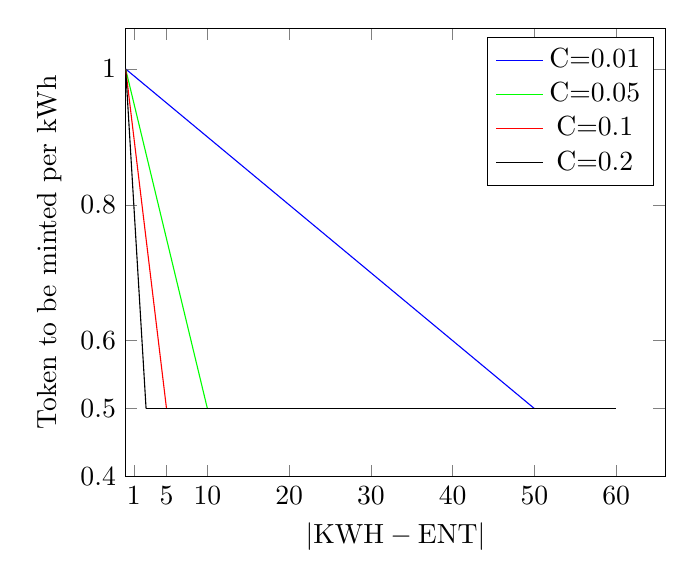
\begin{tikzpicture}
        \begin{axis}[ 
          xlabel=$|\textrm{KWH} - \textrm{ENT}|$,
          ylabel={Token to be minted per kWh},
          xtick={1,5,10,20,30,40,50,60},
          ytick={0,0.2,0.4,0.5,0.6,0.8,1},
          ymin = 0.4,
          xmin = 0
        ]
        \addplot[domain=0:50,color=blue] {1 - x * 0.01};
        \addlegendentry{C=0.01}
        \addplot[domain=0:10,color=green] {1 - x * 0.05};
        \addlegendentry{C=0.05}
        \addplot[domain=0:5,color=red]{1 - x * 0.1};
        \addlegendentry{C=0.1}
        \addplot[domain=0:2.5,color=black]{1 - x * 0.2};
        \addlegendentry{C=0.2}

        \addplot[domain=50:60,color=black]{0.5};
        \addplot[domain=10:60,color=black]{0.5};
        \addplot[domain=5:60,color=black]{0.5};
        \addplot[domain=2.5:60,color=black]{0.5};
        \end{axis}
      \end{tikzpicture}
    \caption{ENT Minting/burning cost for 1 kWh produced/consumed versus the difference between total kWh and total ENT in the network, for different values of C with M = B = 0.5 ENT/kWh}
\end{figure}

The reason we set a cost for minting and burning ENT tokens, is to try to keep the ratio between the total kWh and the total ENT in the network, to 1. Let's consider that for every produced kWh we mint 1 ENT token, in this situation for every $X$ kWh stored we will have $X$ amount of ENT tokens. 
The problem arises when we lose energy due to a potential battery disfunction. In such situation, we will have $Y<X$ kWh available while there are still $X$ amount of ENT tokens in circulation. By applying the minting and burning
functions mentioned above, more tokens will be burned per kWh spent and less tokens will be minted per kWh generated until an equilibrium is reached. This is achieved through the cost function R which adds a cost to every minting 
and burning of ENT tokens in order to keep the total kWh of the storage layer equal to the total ENT in circulation. The constant $C$, defines the percentage of the missing energy to be covered during minting or burning of tokens. The higher the value of the constant, 
the faster equilibrium will be reached but the higher the ENT cost for the individuals, meaning that in practice less network participants are going to cover the loss.\\
The issue with the above mentioned equations, is that we approach equilibrium asymptotically because on each step we cover a fraction of the difference and as we progress that fraction tends to zero. To reach equilibrium in a finite amount of steps and keep the energy loss cost distribution fair, 
the cost $R$ is calculated only when the difference between total kWh and total ENT tokens increase. This means that for every decrease of the difference between these two values, the $R$ value will remain the same until equilibrium is reached or the difference increases again. 
Having this in mind, we calculate the number of kWh $n_t$, that need to be produced or consumed, at a particular time t, until we reach equilibrium, if the difference between the total ENT in circulation and the total available energy in the system, at the time $t$, is $D_t$ and the initial difference that set the cost $R$ is $D_0$. 
\begin{center}
    \begin{math}
        \begin{array}{c}
        D-n_tR = 0 \Rightarrow n_t = \frac{D_t}{R} \Rightarrow\\
    \end{array}
    \end{math}
    \begin{equation}   
        \boxed{n_t = \frac{D_t}{D_0*C}}
        \label{equ:kwh_until_equilibrium}
    \end{equation}
\end{center}
For every kWh produced or consumed, the difference between the total kWh and the total ENT tokens in circulation, is reduced by the cost $R$. This means that after $n_t$ kWh consumed or produced, the difference will be zero.

\subsubsection{Minting/Burning of eEuro tokens}
For the minting of eEuro tokens, a trusted authority is needed. The role of this trusted authority would be to mint new eEuro tokens into the blockchain network as well as burn them. This
task can only be performed by this trusted authority and it is done in a transparent way so everyone in the network can review the validity of the relevant transactions.
For every newly minted eEuro token in the blockchain network, one real world Euro is locked and moved out of circulation. It only exists as its digital version in the blockchain network after the mint
and can be transferred only within the network. When the trusted authority burns the eEuro, it can no longer be used in the blockchain network and real world Euro is unlocked and moved back into circulation.
The network peers can give real world Euro to the trusted authority to mint them the equivalent amount in eEuro and can also burn an amount of eEuro to get real wold Euro back from the trusted authority.
Such a trusted authority could be a certified bank or even a treasury account run by the community.\\
\subsection{Blockchain Layer}
The blockchain layer, is a sub-layer of the information layer, and is where the PowerChain protocol is implemented. On this level, the actual energy and monetary transactions are happening. The PowerChain protocol defines the rules based on which the network tokens are minted,
burned and transferred. It is implemented using a smart contract and thus it is necessary to use a smart contractc apable blockchain platform.
PowerChain uses a private blockchain due to the nature of local energy trading. The decision to use private blockchain was taken because we only want to enable the trade of generated energy locally. A private
blockchain would be more secure in that setup as everyone participating in the network would need to be authorized first by the local community.\\
The blockchain platform we will use for PowerChain is Ethereum with a PoA consensus mechanism. We decided to implement PowerChain on Ethereum due to its active community and because our smart contracts will be directly compatible with the
existing public Ethereum network. In this setup, it could be possible for our local Ethereum network to interact with the public one and enable the trading of energy tokens in a global network. More details on such integration will be
discussed in the next chapters. The decision to use PoA consensus mechanism is to achieve greater stability and security in the network. PoA is also a more suitable fit for a local network with known participants. \cite{manolache2022decision} \\
Despite the fact that we refer to a local community and to local energy trading, PowerChain is not limited to only local energy transactions. It could be possible to initiate transactions between two PowerChain instances of two different
energy trading communities. Different techniques could be explored to connect two private blockchain networks and initiate transactions with one another. More details will be presented on PowerChain integration chapter.

\subsection{Market Layer}
The market layer is where the ENT token exchanges are happening. In order to use the energy stored in the storage layer, consumers need to purchase some ENT tokens from a producer or storage provider.
On the other hand, producers mint ENT tokens by storing energy in the storage layer and would like to sell them for profit. To match these needs, PowerChain has a market platform
where the network participant can access to trade. Consumers submit their offering bit to the market, meaning the price per ENT token they are willing to pay and producers / storage providers submit
their asking bid, meaning the price they would like to be paid per ENT token. For the market clearing the Continuous Double Auction (CDA) mechanism is used. Bids from producers are
ordered from highest to lowest, while bids from consumers from lowest to highest. Then a "price first and time first" principle is applied and the orders are cleared based on the given
bids.\\
Except from the market platform provided by PowerChain, the trade of ENT tokens can happen also by any other mean. It could be possible for two network peers to meet physically and
exchange ENT tokens for cash. It could also be possible to trade the token in another trading platform, assuming that ENT token could be available on that platform. The market layer of PowerChain 
describes any possible way ENT token could be traded in the market and not only the PowerChain market platform.

\subsection{PowerChain Integration} \label{integration}
A PowerChain instance has the possibility to integrate with other PowerChain instances and also with the public Ethereum network. The integration of two remote PowerChain instances enable
the communication of two remote energy trading communities and the exchange of their energy tokens. In such a setup, energy ownership can be transferred between the storage layers of the two
networks and the actual energy transfer can happen through the main power grid by a DSO.\\
There is also the possibility to integrate with the public ethereum network in order to move assets from/to the local PowerChain network. Such assets could be tokens backed by real world currencies
like USDT \cite{Tether}, USDC \cite{CircleUSDC} or EURC \cite{CircleEURC} which could be used for the trading of ENT tokens by the network peers.\\
In order to facilitate such integrations we need to create an smart contract which will be responsible to lock and unlock tokens. This smart contract will be deployed on both networks we need to integrate
and an integration service will be responsible to monitor both smart contracts in order to trigger the unlock of the tokens when necessary.\\
The integration smart contract consists of the following methods:\\
\begin{table}[h!]
\begin{tabular}{c|c|c}
    \textbf{Method}            & \textbf{Description}                                 & \textbf{Callable By} \\
    \hline
                               & Locks received tokens into the contract address.     &                      \\
    \textbf{LockTokens}        & It gets as a parameter the public key of a user      & By any network user  \\
                               & from the other network.                              &                      \\
    \hline
                               & Unlocks or generates tokens into the address of      & Only by the          \\
    \textbf{UnlockTokens}      & a user in the same network. Get as a parameter       & integration service  \\
                               & the public address of the user.                      &                      \\
    \hline
                               & Returns a list of locked tokens along with a public  &                      \\
    \textbf{GetLockedTokens}   & key of a user that belong to the other network       & By any network user  \\
                               & and a unique id representing the lock transaction.   &                      \\
    \hline
    \textbf{TokensTransferred} & Marks a token lock transaction as complete.          & Only by the          \\
                               & Receives as parameter the token lock transaction id. & integration service  \\
\end{tabular}\\
\caption{Methods of integration smart contract}
\end{table}
\begin{figure}[h!]
    \centering
    \includegraphics[scale=0.35]{Figures/PowerChain_Integration.png}
    \caption{PowerChain Integration}
\end{figure}
\\ 
The token transfer between the networks happens in the following stages:
\begin{enumerate}
    \item A user $U_1$ in network $A$, wants to send some tokens to user $U_2$ in network $B$
    \item $U_1$ calls the method \textbf{LockTokens} with the public address of $U_2$ as a parameter and sends $X$ amount of tokens.
    \item The integration smart contract of network $A$ locks the tokens in its contract address and stores the public address of $U_2$ along with the amount $X$
    \item The integration service calls method \textbf{GetLockedTokens} of both network $A$ and $B$ every $T$ seconds
    \item The integration service receives the information that $X$ tokens was locked on network $A$ for the public address of $U_2$ and initiates the \textbf{UnlockTokens} method of network $B$
    \item Tokens are unlocked or generated by the integration smart contract of network $B$ and transferred to the public address of $U_2$
    \item The integration service calls the method \textbf{TokensTransferred} of network $A$ to mark the token transfer as complete.
\end{enumerate}
\pagebreak
\section{Summarization}
In this chapter, we analyzed the main limitations we are trying to address with our proposed architecture and then presented all the components of our solution. We went through the information and physical
layers of the architecture and analyzed the network roles and tokens. We discussed in more details about the minting and burning mechanism of the tokens and delve deeper into the blockchain and market layers.
Finally, we proposed a possible integration architecture that could allow the interconnection of multiple energy trading networks that use our proposed solution. % Framework

\chapter{Implementation and Core Components of PowerChain} \label{platform}
\label{chapter5}
In this chapter we will present the actual PowerChain implementation. We will describe the technical part including what technologies we used and how we used them.
The actual PowerChain implementation along with all the scripts created, can be found at the following GitHub repository:
\begin{center}
    \url{https://github.com/MnAppsNet/PowerChain}.
    \label{code}
\end{center}

\section{Tools Used}
For the implementation of the actual PowerChain network, we used the ethereum client Geth, which is build in the programming language Go.\cite{geth}
Using Bash scripting language, we build some scripts that are leveraging geth to build a PoA network. These scripts can be used to start a new PowerChain network with any number of validators, depending on the network needs.
For security reasons, and only for the validator nodes, we used clef \cite{clef} which is a tool for signing transactions and data in a secure local environment. Clef can be configured with different rules
to authorize transactions and accesses through RPC on the validator nodes to enhance security. For the purpose of this project, the rules are set to allow all connections to the validator nodes through RPC, for testing purposes.
To interact with the PowerChain network, we build some Python scripts using the Web3.py library \cite{Web3py}. These scripts supports us to deploy smart contracts to the network and to call methods of smart contract
instances. We also build a PowerChain web application using React.Js \cite{Reactjs} and the Web3.js \cite{Web3js} library to interact with the blockchain network.\\
The following scripts have been developed to support with the implementation and management of PowerChain network:\\
\begin{table}[h!]
\centering
\begin{tabular}{c|c|p{8cm}}
    \textbf{Script} & \textbf{Type} & \textbf{Desription} \\
    \hline
    pc\_CreateNetwork & Bash & Initiates a guided procedure to setup and initiate a private PoA network with selected number of validators. For each validator a start script is created to start the node. \\
    \hline
    pc\_CreateBootnode & Bash & Initiates a guided procedure to create a bootnode. It creates a start script that can be used to start the node. \\
    \hline
    pc\_CreateAcount & Bash & Initiates a guided procedure to create a user node. It creates a start script that can start the node. \\
    \hline
    pc\_DeployContract & Python & It gets as parameters the path of a solidity smart contract code and the RPC of a node in the network, compiles the contract, deploys it to the network and produces a contract json file that contains the contract address and interface. \\
    \hline
    pc\_CallPowerChainMethod & Python & It gets as parameters the RPC of a node in the network, the path to the PowerChain contract json (json returned from pc\_DeployContract), a method name from PowerChain, the parameters of the relevant method, calls the PowerChain contract and returns the results. It can also be imported on a python script. \\ 
\end{tabular}
\caption{Scripts to create and manage PowerChain network}
\end{table}\\ 

To simulate the production and consumption of energy in and out of a storage unit, we created a python script (storage\_unit.py). 
This script can be used to simulate a storage unit address with capabilities to produce and consume energy. 
In a real life implementation this role will be handled by an IoT device that monitors the input and output of energy to the batteries of a storage unit.

\pagebreak

\section{PowerChain Commands}
The PoweChain protocol defines a set of commands which are implemented into the blockchain layer using a Smart Contract. It determines when and how are the network tokens minted, burned and transferred. 
It also defines the network participant authorizations. In the network, there are different types of roles with each one authorized to execute different type of commands:
\begin{itemize}
    \item \textbf{The normal user}: This is the default role all network participants have. These users can not execute commands that require voting or commands that burn or mint tokens.
    \item \textbf{The voter}: The voters can execute all the commands a normal user is allowed to execute, with the addition of commands that require voting. Such commands could be for example, the promotion of a user to voter
    or the registration of a new storage unit.
    \item \textbf{The storage unit}: This role is assigned to the smart meters managing the energy of a storage unit and it gives the permission to execute commands that lead to the minting or burning of tokens. They
    can also execute normal user commands.
    \item \textbf{The banker}: This role is assigned to the address of a trusted authority which will be responsible to mint/burn eEuro tokens by moving real world euro in and out of circulation.
\end{itemize}
Below, we analyze the commands each of the mentioned roles can execute.\\
\textbf{Voter Commands}:\\
\begin{tabular}{|p{5.5cm}|p{8cm}|}
    \hline
    Register Storage Unit & Start a vote to register a storage unit, providing the unit and the owner addresses \\ \hline
    Remove Storage Unit & Start a vote to remove storage unit, providing the unit address \\ \hline
    Change Banker & Start a vote to register an address as banker, initially the banker address is the zero address \\ \hline
    Set Parameter & Start a vote to set a network parameter, providing the parameter name and value \\ \hline
\end{tabular}\\

\textbf{Storage Unit Commands}:\\
\begin{tabular}{|p{5.5cm}|p{8cm}|}
    \hline
    Energy Produced & Reports energy production based on the producer address and the wh produced \\ \hline
    Energy Consumed & Reports energy consumption based on the consumer address and the wh consumed \\ \hline
    Report Actual Energy & Reports the actual energy that is available in the storage unit  \\ \hline
\end{tabular}\\

\textbf{Banker Commands}:\\
\begin{tabular}{|p{5.5cm}|p{8cm}|}
    \hline
    Mint eEuro & Mint an amount of eEuro into the provided address. \\ \hline
    Burn eEuro & Burn an amount of locked eEuro from the provided address and give the equivalent real world Euro to the user. Only eEuro locked by the user can be burned. \\ \hline
    Unlock eEuro & Unlock an amount of locked eEuro, locked by the user in order to withdraw the relevant real world Euro amount. \\ \hline
\end{tabular}\\

\textbf{Normal User Commands}:
\begin{longtable}{|p{5.5cm}|p{8cm}|}
    \hline
    Get Total Energy & Returns the total energy of the network \\ \hline
    Get Storage Units & Returns the active storage units of the network \\ \hline
    Get Storage Unit Energy & Returns the total energy of a storage unit \\ \hline
    Get Energy Rates & Returns the ENT minting and burning rates of the network \\ \hline
    Start Consumption Session & Start a consumption session with a storage unit for the defined amount of ENT tokens owned by the user \\ \hline
    Get Consumption Session & Returns the consumption sessions of the caller \\ \hline
    Get Consumption Session Energy & Returns the available energy of a consumption session, providing the address of the session counterpart \\ \hline
    Get Storage Unit Info & Returns the state, the owner and the available wh of a storage unit based on its address \\ \hline
    Clear Old Sessions & Clear old sessions that have been expired \\ \hline
    Get Parameters & Returns the network parameters \\ \hline
    Get total ENT & Returns the total amount of ENT in circulation \\ \hline 
    Get total eEuro & Returns the total amount of eEuro in circulation \\ \hline
    Get ENT balance & Returns the amount of locked and unlocked ENT tokens \\ \hline
    Get eEuro balance & Returns the amount of locked and unlocked eEuro tokens \\ \hline
    Transfer ENT & Transfer an ENT amount to the provided address \\ \hline
    Transfer eEuro & Transfer an eEuro amount to the provided address \\ \hline
    Lock eEuro & Lock an amount of eEuro, making burnable by the banker. The banker can then burn the tokens and give the equivalent amount of real world Euro to the user. \\ \hline
    Add Order & Add an order in the orderbook to buy ENT based on required price per unit \\ \hline
    Remove Order & Removes an order from the orderbook \\ \hline
    Get Orders & Returns a list of available orders in the network \\ \hline
\end{longtable}

\section{Network Parameters}
\label{networkParameters}
PowerChain smart contract, defines some parameters that influence the network behavior. These parameters can be modified by the voters, based on the needs of the network participants. 
The mentioned network parameters are the following:
\begin{itemize}
    \item \textbf{M} : Maximum minting cost. This is the maximum ENT cost per kWh to be applied when energy is produced.
    \item \textbf{B} : Maximum burning cost. This is the maximum ENT cost per kWh to be applied when energy is consumed.
    \item \textbf{C} : Missing energy recover rate. This parameter defines how fast will the ration between total energy and total ENT in circulation will return to 1 in case of misalignment.
    \item \textbf{H} : Consumption session validity period. This is the amount of hours a consumption session will remain valid. After the validity period the consumption session is closed and any remaining assets are returned to the owners.
    \item \textbf{F} : Storage provider fee. This is the percentage of the total ENT minted by an energy producer, to be rewarded to the storage provider.
\end{itemize}
These network parameters should be defined carefully in order to incentivize the network peers to participate in the network and provide a fare token distribution.
In case of a big misalignment between the total ENT in circulation and the total energy in the network, parameters M and B are used to make sure that producers are receiving a minimum fare amount of ENT and consumers are not spending too much ENT for their 
energy needs, until the network reaches again equilibrium. Parameter C controls how fast we reach a ratio of 1 between total ENT and total energy, by burning some extra ENT during consumption or minting a fewer ENT during production. A big C value, means that 
we will reach a balance quicker but each individual network participant will have to cover a bigger part of the energy loss through a higher minting/burning cost, potentially splitting the cost to fewer participants. On the other hand, if parameter C is too small, 
the cost to return network in balance is smaller per kWh produced or consumed but network will reach equilibrium slower. Parameter H was introduced to avoid having consumption session assets locked forever. Consumption session will remain valid within the time frame defined by H. 
Finally, parameter F controls what percentage of ENT, from the ENT minted by a producer, should a storage provider keep, for providing its batteries. These parameters have some default values and can be then adapted based on the network needs. The default parameter values are the following:
\begin{itemize}
    \item \textbf{M} = 0.5 ENT / kWh
    \item \textbf{B} = 0.5 ENT / kWh
    \item \textbf{C} = 5 \% of the loss covered each minting / burning (step), equilibrium is reached in at least 20 steps
    \item \textbf{H} = 2 Hours until consumption session becomes invalid
    \item \textbf{F} = 20 \% of minted ENT tokens are kept by storage provider
\end{itemize}

\section{PowerChain Voters}
The PowerChain contract voters have a crucial role in the maintenance and smooth operation of the energy trading network.
They are responsible to audit and agree on the new voters and storage units to be included in the network. They have also
the responsibility to monitor the network and propose new network parameter values that could benefit the participant.\\
As we already mentioned on the previous sections, PowerChain has a set of voter commands. These are a special
kind of commands as they are not directly executable. Every time a voter executes one of these commands, a voting procedure starts with one
positive vote from the voter that executed it. The actual action of the command is not executed until the vote is passed. Whenever another voter 
executes the same command with the same parameters, it agrees with the vote and another positive vote is counted. If the same command with the same parameters 
is executed again by the same voter, the vote changes to a negative vote. For simplicity reasons and in order to keep the voting process fair, we defined that a vote is passed if it has 
more positive votes than the number of voters in the network divided by 2.
\begin{empheq}[box=\fbox]{align}
    \label{equ:vote_pass}
    \text{Vote Passed when: } V_+ / N > 0.5
\end{empheq}
Where,\\
\begin{tabular}{rl}
    $V_+$ & :  Number of positive votes. \\
    $N$   & :  Total number of voters \\
\end{tabular}\\
The voter that adds the last positive vote which  marks the voting as passed, is also executing the action of the command and the voting process is concluded.

\section{PowerChain Web Application}
The PowerChain web application allows the network users to interact easily with the PowerChain contract, though a user interface.
The web application is a control panel that consists of four basic sections and two special ones. To connect the web application with the blockchain network, we make use of MetaMask which works as a blockchain wallet \cite{metamask}.
More details are presented below for each section.
\begin{figure}[h!]
    \centering
    \includegraphics[width=\linewidth,frame,scale=1]{Figures/webapp.png}
    \caption{PowerChain Web Application}
\end{figure}
\begin{itemize}
    \item \textbf{Tokens}: This section provides an overview of the user's tokens and it gives also the possibility to transfer the tokens.
    \item \textbf{Energy}: In this section more information about the network's energy are provided. We can see the available storage units and the amount of energy they contain in kWh.
    There is also the option to start a new consumption session with a storage unit and start consuming energy.
    \item \textbf{Network Info}: In this section more network information are provided to the user like the banker address, the total eEuro in circulation and even the values of the network parameters.
    \item \textbf{Voting}: This is a special section that is only available to the users with the voter role. It provides an overview of the user's votes and gives the possibility to start a new vote.
    \item \textbf{Banker}: This is also a special section that is available only to the banker address. It gives the option to mint, burn and unlock eEuro tokens.
\end{itemize}

\section{Summarization}
In this chapter we went through the core components of our proposed energy trading solution, PowerChain. We discussed about the tools we used to make the implementation happen and the scripts 
we created to help us maintain and manage the PowerChain network. We analyzed the PowerChain smart contract and presented the available commands it offers. We also explored some network parameters that
can influence the network behavior and can be adapted based on the participant needs. Finally, we talked about the voter role defined by the PowerChain protocol and the web application that can be used
to access the PowerChain commands.
 % Platform

\chapter{Experimentation \& Validation} \label{experimentationANDresults}
In this chapter we go through our Network setup and showcase the final implementation. This is a proof of concept implementation with its energy consumption and production functionality simulated.
As future work for this project, PowerChain could be tested against real world production and consumption data or even be implemented as a small scale energy trading network.

\section{Network Setup}
For our network setup, we created a virtual linux Ubuntu environment with the help of PROXMOX \cite{proxmox}.
We used this virtual environment to run our validator nodes. To setup the PowerChain network, we used the script pc\_CreateNetwork which we
created to be able to easily setup a bootnode and the required validator nodes. For our testing purposes, we created a network that submits blocks every second, with two validator nodes that
run on the same virtual environment. In a real life implementation, the different validators must be controlled by different systems and by different users to improve
decentralization. The more validator nodes a network has the better it will be in terms of decentralization. To visualize the block creation and transaction submissions 
to the network, we also setup the Ethereum Lite Explorer by Alethio.\cite{alethio} \\
\begin{figure}[h!]
    \centering
    \includegraphics[width=\linewidth,frame,scale=0.9]{Figures/explorer.png}
    \caption{Example contract method execution transaction on blockchain explorer used with PowerChain}
\end{figure}
After the setup of the network, we need to deploy the PowerChain smart contract that contains all the decentralized functionality of our implementation.
To deploy the contract, we make use of the pc\_DeployContract script that is capable to deploy contracts in the blockchain network. The address that deploys the contract
is automatically given the voter role and is initially the only voter with the power to pass any votes by itself. As a first step for every PowerChain contract instance,
we need to add more voters in order to split the decision making and balance the interests of all parties involved. \\
The next step to finalize the network setup, is to deploy the PowerChain web application that will be used by the network users to interact with the smart contract. 
For our setup, we run the web application in the local network. We now have a working network with the PowerChain smart contract deployed on it and a web application running on
the local network to interact with the contract. The network parameters of the deployed PowerChain contract should have their default initial value (figure \ref{fig:initial_network_state}).
\begin{figure}[h!]
    \centering
    \includegraphics[width=\linewidth,frame,scale=1]{Figures/initial_network_state.png}
    \caption{Initial values for the PowerChain network parameters}
    \label{fig:initial_network_state}
\end{figure}


\section{Testing the PowerChain Contract}
To test the PowerChain contract, we constructed different energy trading scenarios and performed the relevant actions using the PowerChain web application.
Some of these test scenarios are presented in the following sections. Apart from the manual tests performed, we also created some jupiter notebooks that execute
pre-defined tests and checks the results automatically (refer to github address on chapter \ref{code}).

\section{Testing The Voting System}
For this test scenario, we go through the voting system of our PowerChain implementation and test its capabilities.
When the PowerChain contract is initially deployed the only voter in the network is the address that deployed the contract.
At this stage, this address has 100\% of the voting power and can execute any voter command immediately.\\
For this test, we created three blockchain network addresses: 
\begin{itemize}
    \item A = '0xb91ca997c40d6cf4c69ccd3f3c79bcc3ba68b5d0'
    \item B = '0xc7b00cabfb9cc57afd36d52e126aef012e015582'
    \item C = '0x80fc7a6634ea90774a21f43d51d2a84655ff3958'
\end{itemize}
The PowerChain contract is deployed by address A and thus A is automatically assigned the voter role.
As a first action, address A is executing the command 'Add Voter' to make address B a voter. This starts 
a voting procedure which is immediately passed and the action to make address B a voter is executed (figure \ref{fig:voter_added}).
\begin{figure}[h!]
    \centering
    \includegraphics[width=\linewidth,frame,scale=0.7]{Figures/voter_added.png}
    \caption{Address A which has the voter role, assigns successfully the voter role to address B}
    \label{fig:voter_added}
\end{figure}
There are now two voters in the system, this means that in order to execute another voter command, both of them need
to agree. This is because the number of voters is now 2 and in order for the equation \ref{equ:vote_pass} to be valid,
we need at least 2 positive votes.\\
Next step is to also promote address C to a voter. Initially, address B executes the 'Add Voter' command to make address
C a voter but the action is not immediately executed, a voting procedure starts with one positive vote from address B (figure \ref{fig:add_voter_1}).
\begin{figure}[h!]
    \centering
    \includegraphics[width=\linewidth,frame,scale=0.7]{Figures/add_voter_1.png}
    \caption{Address B which is a voter, starts a voting procedure to add the voter role to address C}
    \label{fig:add_voter_1}
\end{figure}
Now it's time for address A to cast its positive vote by executing the command 'Add Vote' to give the voter
role to address C. This will make the voting to pass and the action to be actually executed which means that address C
will now be a voter (figure \ref{fig:add_voter_2}).\\
\begin{figure}[h!]
    \centering
    \includegraphics[width=\linewidth,frame,scale=0.7]{Figures/add_voter_2.png}
    \caption{Address A agrees on the voting to add the voter role to address C and the action is executed}
    \label{fig:add_voter_2}
\end{figure}
For the next step, we need to remove the voter role from address C. For this to happen at least two of the voters has to agree
on this action. Address A and B vote for the removal of address C from voters, the vote is passed and the voter role is revoked from address c (figure \ref{fig:remove_voter}).\\ 
\begin{figure}[h!]
    \centering
    \includegraphics[width=\linewidth,frame,scale=0.7]{Figures/remove_voter.png}
    \caption{Address A and B which have the voter role, agrees to remove the voter role from address c and the action is executed}
    \label{fig:remove_voter}
\end{figure}
Concluding this testing scenario, we see that PowerChain smart contract protects important method executions that can impact the network significantly using
a voting system. Important network changes should be voted and agreed by most of the voters of the network. The voting system of PowerChain is handled automatically
by the smart contracts. This gives the voters freedom to execute commands that changes the network based on their believes. The changes are only truly performed if they 
are also agreed by most of the voters. \\

\section{Testing Energy Production And Consumption}
For this scenario, we will add two new storage units in the network and start producing and consuming energy.
For this purpose, we created the following blockchain addresses:
\begin{itemize}
    \item Voter Address A = '0xB91CA997C40D6CF4C69CCD3F3C79BCC3BA68B5D0'
    \item Voter Address B = '0xC7B00CABFB9CC57AFD36D52E126AEF012E015582'
    \item User Address C = '0x80FC7A6634EA90774A21F43D51D2A84655FF3958'
    \item Storage Unit Address U1 = '0x6E383425169CD23c3eb72709AEf8f81E7847310E'
    \item Storage Unit Address U2 = '0x16E36D7423AD7181B77818462fE0F5Ec5369aEb7'
\end{itemize}
We use the same setup from the previous scenario, so address A and B are already voters. As a first step, the addresses U1 and U2 need to be given the storage unit role to have the possibility to mint and burn
energy tokens (ENT) in the network based on the energy produced and consumed. To do so, voter A and voter B need to start two voting
sessions, one to give the address U1 the storage unit role and another one for U2. We will define as the owner of both storage units, the
user address C. As we only have two voter, both have to agree for the votes to pass (figure \ref{fig:add_units}).\\
\begin{figure}[h!]
    \centering
    \includegraphics[width=\linewidth,frame,scale=1]{Figures/add_units.png}
    \caption{Address A and B which have the voter role, vote for the addition of two new storage units. The last two votes in the image represent the vote for the addition of the new storage units.}
    \label{fig:add_units}
\end{figure}
Now that we have two storage units in the network that are owned by user address C, the peer with address A, produces 10 kWh in the storage unit U1. The storage unit U1
reports the production to the blockchain and the relevant ENT tokens are minted. We simulate the energy production reporting using a python script (storage\_unit.py). In a real world scenario, there should be
a smart meter (an IoT device) that controls the storage unit address. This device is responsible to monitor the inbound/outbound energy and report relevant production and consumption of energy to the blockchain network.
After the production of 10 kWh from address A in the storage unit U1, address A should be rewarded with 8 ENT and the address C with 2 ENT. 
That's because the storage unit U1 belongs to user with address C and the storage provider fee parameter is set to 20\%.
As for the storage unit U1, it should now have 10 kWh available (figure \ref{fig:energy_produced}).\\
\begin{figure}[h!]
    \centering
    \includegraphics[width=\linewidth,frame,scale=1]{Figures/energy_produced.png}
    \caption{Overview of the web application information provided to address A after the energy production}
    \label{fig:energy_produced}
\end{figure}
For the next step, user with address C wants to consume some of the energy of storage unit U1. It has 2 ENT available which were received from the energy production of address A as a storage provider fee.
It starts a consumption session with unit U1 for 2 ENT which corresponds to an energy consumption of 2 kWh as there is no burn cost currently in the network.
With the consumption session of 2 kWh active, user address C consumes 1 kWh and unit U1 reports it. At this stage, user address C should have 1 locked ENT (the other one was consumed) and the storage unit U1
should have 8 kWh available, 1 already consumed and another one locked in the consumption session with user address c. The total ENT in circulation should be reduced to 9 and the same should happen also to the
total energy in the network (figure \ref{fig:consumption_session}).\\ 
\begin{figure}[h!]
    \centering
    \includegraphics[width=\linewidth,frame,scale=1]{Figures/consumption_session.png}
    \caption{Consumption session of user address C before (left side) and after (right side) the consumption.}
    \label{fig:consumption_session}
\end{figure}
Proceeding further, we will study the case when the user address C consumes more kWh than were locked in the consumption session. This could happen due to an issue with the energy consumption monitoring of the smart
meter for example, which might allow the consumer to consume more than what was agreed with in the consumption session. In this case, we will have an imbalance in the system which will lead in a minting and burning
cost for the network, in order to counteract it. User address C has now 1 kWh left in the consumption session with unit U1 but due to a malfunction, 2 kWh were consumed. Unit U1 reports this consumption and the network will now have
8 ENT but only 7 kWh in total. The consumption session with user address C is terminated (figure \ref{fig:energy_imbalance}). \\
\begin{figure}[h!]
    \centering
    \includegraphics[width=\linewidth,frame,scale=1]{Figures/energy_imbalance.png}
    \caption{Due to network energy imbalance, a burning and minting cost is applied. The above image is an overview of the information provided to user address C.}
    \label{fig:energy_imbalance}
\end{figure}
The PowerChain smart contract will try to balance the ration between total ENT tokens and total kWh by applying a cost to each mint and burn of ENT tokens. Using the equation \ref{equ:kwh_until_equilibrium}, we can calculate when
equilibrium will be reached:
\begin{math}
    n_0 = \frac{D_0}{D_0*C} \Rightarrow n_0 = \frac{1}{C} \Rightarrow n_0 = 20 kWh
\end{math}.
So in the next 20 kWh that will be produced or consumed, the network will reach equilibrium. To study this behavior, we first produce 10 kWh from address B into storage unit U2.
This will reduce the difference to $D_{t1} = D_0 - 10*R \Rightarrow D_{t_1} = D_0 - 10*D_0*C \Rightarrow D_{t_1} = 0.5$. From this energy production $E_p$, the ENT tokens minted $\textrm{ENT}_{mint}$, based on the
minting cost $R=D_0*C=0.05$, are $\textrm{ENT}_{mint}=E_p*(1-R) \Rightarrow \textrm{ENT}_{mint}=10-10*0.05=9.5 ENT$. Due to the storage provider fee $F$, the ENT tokens received by
address B, are $\textrm{ENT} = \textrm{ENT}_{mint} - \textrm{ENT}_{mint} * F = 7.6 ENT$ (figure \ref{fig:reduce_imbalance}).\\
\begin{figure}[h!]
    \centering
    \includegraphics[width=\linewidth,frame,scale=1]{Figures/reduce_imbalance.png}
    \caption{After the production of 10kWh, the energy imbalance is reduced. In this figure we see the information provided to address B.}
    \label{fig:reduce_imbalance}
\end{figure}
As a final step for this scenario, we try to resolve the imbalance with an energy consumption worth of 15.6 ENT. To do so, address B transfers
its 7.6 ENT tokens to address A in order for address A to have 15.6 ENT available. Address A starts a consumption session for 7.35 ENT with unit U1 
and for 8.25 ENT with unit U2. Based on the burn cost, this is equivalent to $7.35/(1+R) = 7 kWh$ for the consumption session with unit U1 and 
$8.25/(1+R) = 7.857 kWh$ for the consumption session with unit U2. Address A consumes initially the 7 kWh from unit U1 and the storage unit reports the
consumption to the blockchain network. This will result in reduction of the difference between the total ENT and available energy to $D_{t_2} = D_0 - 17*R \Rightarrow 
D_{t_2} = D_0 - 17*D_0*C \Rightarrow D_{t_2} = 0.15$ (figure \ref{fig:reduce_imbalance_2}).
\begin{figure}[h!]
    \centering
    \includegraphics[width=\linewidth,frame,scale=1]{Figures/reduce_imbalance_2.png}
    \caption{Address A starts a consumption session with unit U1 and U2 (left side) and then consumes 7 kWh from storage unit U1 (right side).}
    \label{fig:reduce_imbalance_2}
\end{figure}
To cover the final difference $D_{t_2} = 0.15$ and reach equilibrium, we need to consume or produce another $n_{t_3} = \frac{D_{t_2}}{D_0*C} = 3 kWh$. To do
so, address A consumes the final 7.857 kWh from the consumption session with unit U2. From these 7.857 kWh, $E_e=3$ kWh will be consumed with ENT burning cost of 0.05 ENT/kWh
and the rest with no cost because after the 3 kWh, equilibrium will be reached and the cost $R$ will be set to 0. This means that the ENT to be burned from this energy
consumption are $\textrm{ENT}_{burn} = 3*(1+R) + (E_c-3) = 8.007 ENT$. For that reason $8.25 - 8.007 = 0.243 ENT$ will be returned back to address A because initially 8.25 ENT were
locked in this consumption session (figure \ref{fig:resolve_imbalance}). \\
\begin{figure}[h!]
    \centering
    \includegraphics[width=\linewidth,frame,scale=1]{Figures/resolve_imbalance.png}
    \caption{This this figure we see the information provided to address A after the consumption of the energy from the consumption session with unit U1. The imbalance between the total
    ENT in circulation and the available kWh in the network is resolved.}
    \label{fig:resolve_imbalance}
\end{figure}
Concluding this test scenario, we see that the PowerChain smart contract is able to handle energy consumption deals between the network users and the storage units. It is also capable to automatically 
handle imbalances between the available energy in the network and the ENT in circulation, by applying a minting and burning cost. The automatic balancing mechanism is important to keep the ENT token 
tethered to the value of a particular amount of energy which is 1 kWh is our case.

\section{Testing the market layer}
In this testing scenario, we test the market layer of the PowerChain contract. For this test we use the same addresses with the previous testing scenario. In the current state of the network,
address A has 0.243 ENT tokens and address C has 1.9 ENT tokens. In order to use the market layer, we need to introduce the banker role in our network. The banker role will allow us to mint 
eEuro tokens that can be used to buy and sell ENT tokens. For this purpose, voter address A and voter address B agree on giving the banker role to address C (figure \ref{fig:new_banker}).
\begin{figure}[h!]
    \centering
    \includegraphics[width=\linewidth,frame,scale=0.7]{Figures/change_banker.png}
    \caption{In this figure we see the information provided to address A. The banker address has been changed to user address C.}
    \label{fig:new_banker}
\end{figure}
Address C can now move eEuro tokens in and out of circulation by minting and burning them. In a real world case, this role should be assigned to a trusted third party that will be responsible
to lock real world EUR and mint the relevant amount of eEuro in the PowerChain network. It is also responsible to unlock real world EUR and burn the relevant amount of eEuro, so the network users
can withdraw their eEuro. For the purposes of this test scenario, address C mints 10 eEuro into address A (figure \ref{fig:eEuro_minted}).\\ 
\begin{figure}[h!]
    \centering
    \includegraphics[width=\linewidth,frame,scale=0.7]{Figures/eEuro_minted.png}
    \caption{In this figure we see the information provided to address A. The banker address has been changed to user address C.}
    \label{fig:eEuro_minted}
\end{figure}
Address C has 1.9 ENT available and starts a sell order with cost 0.5 eEuro/ENT. Address A wants to buy 10 ENT with cost 1 eEuro/ENT and creates the relevant order in the market.
The system matches the buy order of address A with the sell order of address C and 1.9 ENT tokens are bought from address A for a total of 0.95 eEuro. This will reduce the requested
amount of the buy order of address A to 8.1 ENT with requesting price of 1 eEuro/ENT (figure \ref{fig:order_book}).\\ 
\begin{figure}[h!]
    \centering
    \includegraphics[width=\linewidth,frame,scale=1]{Figures/order_book.png}
    \caption{In this figure we can see the sell order created by address C (on the left side) and the buy order created by address A (on the right side) which automatically consumed the sell
    order of address C}
    \label{fig:order_book}
\end{figure}
Concluding this test scenario, we see that the PowerChain smart contract can automatically match the buy and sell orders of the users, using an order book style CDA market. This market maker mechanism
is very simplistic and could be enhanced to improve the user experience and possibly provide a unified energy price.

\section{Comparison with literature}
Based on our exterminations, it is apparent that PowerChain is a viable energy trading solution but how does it compare against the literature implementations we studied on chapter \ref{chapter3}?
In the following table we summarize the main aspects of the studied solutions along with our proposed one.
\newcolumntype{Y}{>{\centering\arraybackslash}m{2cm}}
\begin{table}[h!]
    \centering
    \begin{tabularx}{\textwidth}{|Y|Y|Y|Y|Y|Y|}
        \hline
        \textbf{Aspect}         & \textbf{PowerChain} & \textbf{\hyperref[sec:hfi]{A Frabric implementation}}      & \textbf{\hyperref[sec:dtr]{DeTrade}} & \textbf{\hyperref[sec:nrgc]{NRGCoin}} & \textbf{\hyperref[sec:cda]{Energy trading on CDA market}} \\
        \hline
        \textbf{Blockchain}     & Private Ethereum & Private Hyperledger Fabric & Private Hyperledger Burrow & Public Ethereum  & Public Bitcoin \\
        \hline
        \textbf{Consensus}      & PoA & BFT & BFT & PoS & PoW \\
        \hline
        \textbf{Market}         & Open Currency exchange with a CDA implementation on top & MCP (average buy offer) & DeMarket (pool-based) & Open currency exchange & CDA \\
        \hline
        \textbf{Energy Consumption} & Indirect, backed by ENT token & Direct, energy consumed at the time of production & Direct, energy consumed at the time of production & Indirect, backed by NRGCoin & Direct, energy consumed at the time of production \\
        \hline
        \textbf{Need for energy forecast} & No & Yes & Yes & No & Yes \\
        \hline
        \textbf{Relying on DSO and current energy transfer model} & Not if there is enough energy storage capacity in the network & Yes in case of energy contract breach due to forecast error & Yes in case of energy contract breach due to forecast error & Yes as it sends the produced energy to local substations & Yes in case of energy contract breach due to forecast error \\
        \hline
    \end{tabularx}
    \caption{Comparison of energy trading network from literature with PowerChain}
\end{table}\\ 
Compared to the models that follow a direct energy consumption architecture, approves upon the following points:
\begin{itemize}
    \item There is no need for energy forecasts giving the possibility to network participants to decide when and how much energy they need to consume or produce.
    \item There is no dependency on the traditional energy market and the DSOs as long as there is enough energy storage capacity on the network. Direct consumption approaches are always depended on the traditional energy market as there is always
    the risk of a forecast mistake which can lead to breaches to energy trading agreement and thus any excess energy produces or any additional energy consumption need to be covered by the traditional means.
    \item There is more freedom on when and how much energy to be consumed as the consumption and the production can happen asynchronously.
\end{itemize}
Compared to NRGCoin which uses the existing traditional energy transfer equipment to store energy, following an indirect energy consumption architecture, PowerChain introduces a local network energy storage layer. In that way, it decouples from the traditional energy
transfer model providing more freedom to its participants when it comes to how they want to maintain approve upon their network. Additional the energy market is formed only based on the participant needs and can't be immediately influenced by a DSO.

\section{Summarization}
In this chapter we examined our proof of concept PowerChain implementation by testing it against different scenarios. We tested the voting system of PowerChain by adding and removing voters in the network, the handling of energy consumption/production by the PowerChain
protocol and how an energy imbalance is handled automatically by the protocol through ENT minting and burning costs. We also tested the CDA energy trading market implemented in the PowerChain smart contract by creating some buying and selling orders of ENT tokens. Finally, we compared
the energy trading implementations of literature with our proposed solution and highlighted the points we are improving upon. % Experimentation

\chapter{Conclusions \& Future Work} \label{conclusions}
This research successfully implemented a decentralized energy trading model called PowerChain, utilizing a private blockchain network. 
The results demonstrate the feasibility of our model in facilitating secure, transparent, and traceable energy asset exchanges within a local network.
Using a private blockchain network with known participants we reinforce the security aspect of the implementation. By nature of blockchain technology we
achieve transparent and traceable energy asset exchanges as every transaction in the network is known and visible to all participants. Like the rest of the P2P
energy trading implementations in literature, PowerChain addresses effectively the problems that arise from the traditional energy market (refer to section \ref{problems})
and improves upon existing literature by introducing a novel architecture.

\section{PowerChain Novelty}
In comparison with existing energy trading models in literature that leverages blockchain technology, PowerChain offers some unique characteristics.
It introduces a novel framework incorporating the energy storage layer and storage provider concept. 
The primary challenge it tries to tackle, is related to the error-prone forecasts required by direct energy consumption architecture which is prevalent among solutions in literature. 
Apart from the fact that forecasts can be susceptible to errors, tt could also be that producers or consumers try to manipulate the energy market by purposely 
providing false energy predictions. The introduction of the energy storage layer can resolve these issues as there is no need for energy forecasts anymore.
Producers are getting rewarded to provide energy to the energy storage layer and consumers buy from the already available energy of the network. Although this solution
tackles efficiently the energy forecasting issues, it comes also with its challenges. 

\section{PowerChain Challenges and Limitations}
The main challenge of PowerChain is the fact that storage units need to maintain large batteries for the storage of energy. The storage layer of the network need to have sufficient energy 
storage capacity for the network needs and constantly increase it based on the demands. This brings a high cost on the setup and maintenance of the network. PowerChain tries to tackle this 
challenge by applying a storage provider fee, to incentivize users to provide energy storage to the network. Its biggest limitation is the reliance on batteries for the energy trades 
and the high cost this introduces to the network setup and maintenance. With the advancements of battery technology, these costs could be reduces and the energy could be stored more efficiently with higher
energy density batteries.\\ 

\section{Future Work}
In this section we are highting some open topic of this study that could be research material for future work. Below we enumerate these topics and describe them in more details.
\begin{enumerate}
    \item Research on the implementation of the smart meters that are responsible of reporting energy consumption and production events to the PowerChain smart contract.
    \item Integration of PowerChain networks with each other and this existing public EVM compatible blockchains.
    \item Investigation into the bridging of legal currencies into the private PowerChain network.
    \item Investigate the possibility of implementing a hybrid architecture that allows for both direct and indirect energy consumptions.
    \item Research on the current state of battery technology and the actual cost to setup and maintenance a network leveraging PowerChain architecture.
\end{enumerate}
\subsection*{Smart Meters}
While PowerChain was proven to be a feasible energy trading model theoretically, more research is needed to practically implement it in a real world scenario.
Our research was mostly focused on the blockchain layer and the handling of network assets but there is also more investigation needed on the
physical devices that can implement the model in practice. One such device is the smart meter which is an IoT device, controlling a blockchain address, 
responsive to monitor energy production/consumption and report them to the blockchain network. It is a very important part of the network
because it works as an interface between the digital assets and the actual energy movements. More research is needed on how to setup such
devices and how to make sure that the metrics they report can not be tampered with and will always represent the actual metrics with a sufficiently high accuracy.
\subsection*{PowerChain Integration}
Another aspect that need to be studied further, is the integration of a PowerChain network instance with other remote instances or even with other public EVM compatible blockchains.
In this study we presented an initial draft of an integration solution, in chapter \ref{integration}, but more investigation is needed about its feasibility. The integration of a PowerChain instance
with other instances will open the doors to energy trade deals between energy communities, allowing to export and import energy to each other. The option to integrate with
public blockchains will allow the bridging of existing assets from the public blockchain into the local PowerChain network. Such asset could be a stable coin that can be used
for the trading of ENT tokens and thus avoid putting trust in a trusted authority to bring EUR assets into the network.
\subsection*{Bridging legal currencies into the private network}
Additional investigation is also needed on the bridging of real world currencies into the private blockchain network. The banker role, introduced in the PowerChain protocol to bridge currency assets into
the private network, has a lot of power and could potentially exploit the network. An improvement on top of the banker role, would be the implementation of a community fund powered by the voter role and thus
network voters would collectively agree on the minting and burning of currency assets.
\subsection*{Investigation of hybrid solutions}
The merging of direct and indirect energy consumption architectures would also be an interesting study subject. The integration of direct energy consumption on top of the indirect one proposed by PowerChain,
could help mitigate some of the limitations of both architectures. Network peers could rely on energy forecast for the energy trades and a storage layer could provide a backup when a contract is breached due to
forecasting errors. In addition direct energy trades could help reduce some of the battery related costs by reducing the required network storage capacity.
\subsection*{State of battery technology and the costs to setup a PowerChain network}
While in theory PowerChain seems like a good solution for implementing a P2P energy trading network, more research is needed on the costs related to a practical setup of the network. The current state of battery technology
need to be investigated along with the efficiency, energy density and cost of state of the art batteries. In addition, there is the need to collect and analyze real world energy consumptions of a local community in order to
understand what is the required energy storage capacity of a PowerChain network and what are the costs related to purchasing and maintaining the relevant amount of batteries. Based on the results of such a study, we can
calculate what would be the most appropriate values for the PowerChain network parameters (refer to section \ref{networkParameters}) in order to incentivize all network peers to continue using and improve upon the network.
 % Results and Discussion

%\input{Chapters/Chapter7} % Conclusion

%% ----------------------------------------------------------------
% Now begin the Appendices, including them as separate files

\addtocontents{toc}{\vspace{2em}} % Add a gap in the Contents, for aesthetics

\appendix % Cue to tell LaTeX that the following 'chapters' are Appendices

% \chapter{Example Appendix} \label{math}
 
% Example appendices

\addtocontents{toc}{\vspace{2em}}  % Add a gap in the Contents, for aesthetics
\backmatter % End the book's numbering; backpage

%% ----------------------------------------------------------------
\label{Bibliography}
\lhead{\emph{Bibliography}}  % Change the left side page header to "Bibliography"
\bibliographystyle{ACM-Reference-Format}
% \bibliographystyle{unsrtnat}  % Use the "unsrtnat" BibTeX style for formatting the Bibliography
\bibliography{Bibliography}  % The references (bibliography) information are stored in the file named "Bibliography.bib"

\end{document}  % The End
%% ----------------------------------------------------------------